\documentclass[DM,lsstdraft,toc]{lsstdoc}
\usepackage{graphicx}
\usepackage{url}
\usepackage{color}

\title[Photo-$z$ for LSST Objects]{Options for Photometric Redshifts for the LSST Data Release {\tt Object} Catalog}

\author{M.~L.~Graham, J.~Bosch, L.~P.~Guy, (ADD MORE), and the DM System Science Team.}

\setDocRef{DMTN-049}
\date{\today}
\setDocRevision{TBD}
\setDocStatus{draft}

\setDocAbstract{
This document discusses options for the generation and validation of photometric redshifts for the LSST Data Release {\tt Objects} catalog.
This is a {\it living document} which will progress over time as the photo-$z$ attributes are defined, one or more estimators are selected, and the validation process is established.
Contributions from the science community are solicited regarding the contents of this document.
}

\setDocChangeRecord{%
\addtohist{1}{2017-04-01}{Initial release of preliminary investigation.}{Melissa Graham}
\addtohist{2}{2018-10-16}{Edited to align with recent DPDD updates, some of which were based on the recommendations of Version 1 of this document.}{Melissa Graham}
\addtohist{3}{2019-XX-XX}{Updated as per ticket/DM-6367.}{Melissa Graham}
}

\begin{document}

\maketitle

% CITATION EXAMPLES
% \verb|\citellp|: \citellp{LPM-17, LSE-30} \\
% \verb|\citell|: (SRD; \citell{LPM-17,LSE-29}) \\
% \verb|\citep[][]|: \citep[e.g.,][are interesting]{LPM-17,LSE-29} \\
% \verb|\cite|: \cite{LPM-17,LSE-29}



% % % % % % % % % % % % % % % % % % % % % % % % % % % % % %
\section{Introduction} \label{sec:intro}

A {\it photometric redshift} is an estimate of an object's cosmological redshift (distance) which is based on its photometry (e.g., apparent magnitudes in multiple filters) instead of on its spectral features (e.g., emission and absorption lines). 
Redshift (distance) is a key component of many science goals that will be pursued with the LSST data.
Since it will be impossible to obtain spectra for the billions of galaxies that LSST will observe, photometric redshift estimates will be necessary.

Typically, photometric redshift estimators either fit template spectra to the observed photometry or match photometry to a training set of galaxies with spectroscopic redshifts. 
The latter is often done with machine learning codes, and hybrid photo-$z$ estimators also exist. 
Some photo-$z$ estimators are more appropriate for some science goals than others, due to the quality or type of results they produce (e.g., point estimates, full posterior probability density functions, PDFs, or redshift distributions in tomographic bins).
For this reason, several research groups in the science community are already planning to generate multiple kinds of photo-$z$ (e.g., the Dark Energy Science Collaboration).

However, it would be scientifically prohibitive if all LSST users had to generate their own photo-$z$ estimates, as this is a computational intensive calculation.
Furthermore, it is a requirement\dmreq{0046} that the LSST Data Management System (DMS) calculate photo-$z$ and store them in the {\tt Object} catalog.
Research and development of photometric redshift algorithms for LSST is beyond the scope of DM (not part of DM's specialized knowledge base), as it is itself an active area of current and future LSST research.
Instead, one or more existing photo-$z$ estimator(s) would be installed by DM into the DR pipeline and run at scale, and/or a user-generated photo-$z$ catalog could be ingested and federated with the {\tt Object} catalog.

{\bf The purpose of this document} is to clarify how the DMS will fulfill the requirement to generate and serve {\tt Object} photo-$z$ with each data release during Operations; to define the attributes and performance of this data product, as well as its associated documentation; and to describe how contributions from the LSST science community, which has a considerable wealth of expertise in generating photo-$z$ catalogs, will be incorporated.


\clearpage
% % % % % % % % % % % % % % % % % % % % % % % % % % % % % %
\section{Proposed Timeline}\label{sec:time}

The following is a proposed path to prepare the DMS to generate and serve {\tt Object} catalog photo-$z$ as part of the data release processing pipeline during Operations.

\subsection{Q4 2020: Define Minimum Attributes}\label{ssec:time_mvp}

A preliminary proposal for the minimum attributes (e.g., the type, outputs, performance) of the {\tt Object} catalog photo-$z$ is put forth in \S~\ref{sec:mvp}.
Community input on the definition of these attributes will be solicited via the science collaborations and through interaction at meetings.
This iterative process should end by Q4 2020, when the LSST Project will update to this document with the definition of photo-$z$ attributes. 

{\bf Estimated Level of Effort:} \textcolor{red}{2 months FTE (DM Science Analyst).}

\subsection{Q4 2021: Select Algorithm(s)}\label{ssec:time_sel}

A preliminary proposal for the process by which potential photo-$z$ algorithms should be evaluated and selected is put forth in \S~\ref{sec:sel}.
Community input on the selection criteria and the benefits/drawbacks of potential algorithms will be solicited via the science collaborations and through interaction at meetings.
This iterative process should end by Q4 2022, when the LSST Project chooses one or more algorithms to be implemented, and updates this document with the details of the selection.

{\bf Estimated Level of Effort:} \textcolor{red}{2 weeks FTE (sum of all Project staff involved in decision process).}

\subsection{Q4 2023: Implementation into the DMS}\label{ssec:time_impl}

The DM team is responsible for implementing the chosen algorithm(s) into the data release pipeline, along with any needed supporting data sets (e.g., templates, spec-$z$ catalogs) and the related validation codes. A preliminary proposal for the elements of photo-$z$ validation are assembled in \S~\ref{sec:val}, and lists of data products associated with photo-$z$ are collected in \S~\ref{sec:dp}. Community assistance with the process of implementing the photo-$z$ algorithm and its validation codes will be solicited via the science collaborations and through interaction at meetings, and might include access to commissioning data or DR previews\footnote{\textcolor{red}{DR previews are currently envisioned to be some small, e.g., $\sim10\%$, amount of a data release made available early, e.g., weeks to months, before the full DR to enable community feedback. FIND THE RIGHT DOC TO REF FOR DR PREVIEWS.}}.
This process should end by Q4 2023 or the start of Operations.

{\bf Estimated Level of Effort:} \textcolor{red}{0.5 years FTE (DM developer).}

\subsection{Data Release}\label{ssec:time_dr}

The DMS produces and validates photo-$z$ for the {\tt Object} catalog, and these photo-$z$ are available at the time of data release during LSST Operations, along with any and all supporting materials such as documentation or spectral templates.
The LSST Operations project may solicit and collect community feedback on the photo-$z$, and return to any stage of this path and change the attributes, algorithm, implementation, and/or validation of {\tt Object} catalog photo-$z$ for future data releases.

{\bf Estimated Level of Effort:} \textcolor{red}{0.5 years FTE, and then 1 month per year throughout Operations (DM developer).}

\subsection{Option: Federate a Community Photo-$z$ Catalog}\label{ssec:time_opt}

As described in this document, the DMS as delivered to the Operations Project will provide a minimal scientific capability with respect to {\tt Object} catalog photo-$z$, but if that is rendered obsolete by community efforts, then the superior product should be ingested and federated.

To facilitate this option might require providing the community team(s) with access to DR previews so that they may train and calibrate their photo-$z$ algorithm, and minimize the time between data release and federation of a new photo-$z$ catalog to the {\tt Objects} table.

Options to federation and integration into the {\tt Objects} catalog might include, for example, the LSST Operations agreeing to host a "photo-$z$ server" within the LSST Science Platform. For example, a system like the Dark Energy Survey's Science Portal to serve photometric redshifts \cite{2018A&C....25...58G}. \textcolor{red}{Placeholder for citation of a future document about federating data products.}

{\bf Estimated Level of Effort:} \textcolor{red}{2 weeks FTE (DM developer).}

\subsubsection{The Science Impact of a DR Without {\tt Object} Photo-$z$}

This option to federate a community-generated photo-$z$ catalog leads to this question: {\it if there will likely be a superior community photo-$z$ anyway, could the project simply wait and then use that?} However, there are several significant risks and drawbacks to this option.
\vspace{-15pt}
\begin{itemize}
\item An {\tt Object} table without photo-$z$ at the time of data release is a problem for brokers, unless alerts are instead (or additionally) associated to an older DR's {\tt Object} catalog that has photo-$z$. Brokers require host-galaxy photo-$z$ to optimally classify and prioritize transients for follow-up, and plan to obtain this information via each alert's associations with nearby {\tt Objects} from {\it the most recent DR}.
\item This option does not satisfy the requirement that the {\it "DMS shall compute"} photo-$z$, as it is currently worded.
\item The {\tt Object} photo-$z$ might be tailored to the specific science case of the community team and might not serve the broader science use-cases.
\item There is no initiative or reward for the community team which has generated the photo-$z$, except perhaps citations to their photo-$z$ catalog.
\item There would be no {\tt Object} photo-$z$ if no community team generates and donates a catalog, which is a risk for the science use-cases described in \S~\ref{ssec:use_sci}
\end{itemize}

%% % % % % % % % % % % % % %
%\subsection{Mario's Original Roadmap to Photo-$z$}\label{ssec:dmcalc_mario}
%This option has served as the basis for our discussions with the science community since 2016, and is based on comments by Mario Juri\'{c} on the Jira thread DM-6367.
%The process for the definition of the Data Release (DR) photo-$z$ data product is:
%\begin{enumerate}[noitemsep,topsep=-10pt]
%\item DM Project Science (acting on behalf of overall Project Science) consults with the community (represented by the relevant collaboration -- in this case, the DESC) for proposed options regarding the most appropriate algorithm and format for the results. Iteration between DM and the science community will be necessary in order to converge to a scientifically acceptable {\it and} implementable solution (e.g., if DESC recommends an algorithm that does not meet DM's computational, storage, or budget limitations, or if DESC recommends an algorithm that the other SC have concerns with).
%\item Following that (iterative) consultation, DM will recommend (and the Project will select) the photo-$z$ algorithm and the data product format to be incorporated into DR Processing.
%\item DM will implement the selected algorithm, using whatever they can transfer over from DESC (or other) work, but DM's requirements may be higher than DESC's (e.g., the algorithm will need to run reliably in LSST's production environment).
%\item DM will implement anything needed to integrate, verify, validate, and run QA on the photo-$z$ data product in data releases (and everything leading up to the annual releases; e.g., commissioning), because photo-$z$ are ultimately a Project deliverable.
%\end{enumerate}

\clearpage
% % % % % % % % % % % % % % % % % % % % % % % % % % % % % %
\section{Proposed Minimum Attributes}\label{sec:mvp}

\textcolor{red}{As described in \S~\ref{sec:time}, these proposed minimum attributes will be refined via interaction with the broader scientific community.}

The DMS-generated {\tt Object} photo-$z$ should, at minimum, {\it meet the basic science needs for communities which will not or cannot generate custom photo-$z$}, and also DM's internal use-cases. The basic science needs and use-cases for {\tt Object} photo-$z$ which were used to propose this set of preliminary minimum attributes are described in \S~\ref{sec:use}.

A {\it basic} science need would not include, for example, photo-$z$ of the quality required for major cosmological advances.
The development of such photo-$z$ algorithms is an active research topic within the Dark Energy Science Collaboration \cite{2018arXiv180901669T}, and a significant effort which the LSST Project should not (and could not) attempt to replicate. 

% Preliminarily, it seems very likely that off-the-shelf photo-$z$ estimators will be able to fulfill these basic necessities (as discussed in \S~\ref{sec:sel}).

{\bf Type of Algorithm}\\
The {\tt Object} catalog photo-$z$ should be based on a template-fitting algorithm {\it and then also} a machine-learning algorithm, if multiple results can be stored (see \S~\ref{ssec:dp_store}).
The main motivation for this is galaxies-related science (\S~\ref{sssec:use_sci_gal}) and internal (\S~\ref{ssec:use_dm}) use-cases, which would use the best-fit template to derive additional galaxy properties.

{\bf Output Format}\\
The {\tt Object} catalog photo-$z$ should include the posterior distribution function and a point estimate with an uncertainty, as well as reliable uncertainties and/or flags to help the novice user avoid mis-applying the results, or over-estimating their significance.
For template-fit photo-$z$ results, an identifier for the best-fit template should be provided, and those templates be made publicly accessible.
A list of the photo-$z$ outputs (and documentation) is put forth in \S~\ref{ssec:dp_pz}.

{\bf Performance}\\
The {\tt Object} catalog photo-$z$ could have a point-estimate accuracy of $\sim10\%$ and still meet the basic science needs.
The photo-$z$ results should have a standard deviation in $z_{\rm true}-z_{\rm phot}$ of $\sigma_z < 0.05(1+z_{\rm phot})$, and a catastrophic outlier fraction of $f_{\rm outlier} < 10\%$, over a redshift range of $0.0 < z_{\rm phot} < 2.0$ for galaxies with $i<25$ mag galaxies.



\clearpage
% % % % % % % % % % % % % % % % % % % % % % % % % % % % % %
\section{Proposed Selection Criteria} \label{sec:sel}

\textcolor{red}{As described in \S~\ref{sec:time}, these proposed selection criteria will be refined via interaction with the broader scientific community.}

Criteria to be used in the selection of one or more photo-$z$ algorithms by the LSST Project. These criteria may also apply to community-generated catalogs proposing to be federated with the {\tt Objects} table (or be otherwise served at scale to the broader science community).

{\bf Minimum Attributes}\\
Whether the algorithm meets the minimum attributes defined in \S~\ref{sec:mvp}, and can meet {\it the basic science needs} as well as internal use-cases.
Performance beyond the basic needs, and the ability to provide higher-quality photo-$z$ results, should also be considered.
Statistical methods to assess and compare the photo-$z$ performance from a variety of algorithms are discussed in \S~\ref{sec:eval}.
The proposed minimum performance is likely achievable for LSST data with current photo-$z$ estimators, as demonstrated in \S~\ref{ssec:eval_ex}.

{\bf Scientific Utility}\\
The selected algorithm(s) should serve as wide a variety of science needs as possible.
Demonstrated success with other wide-field optical surveys, previous application to surveys that overlap with LSST (for results comparisons), and general community support or adoption of the estimator should all be considered.

{\bf User Experience}\\
The photo-$z$ estimator's algorithms and output should be straightforward to understand and easy to access.
The selected algorithm(s) should have detailed, publicly accessible documentation (e.g., a journal article, a website, a schema) to facilitate community use.
Desired photo-$z$ outputs, access methods, and documentation are discussed in \S~\ref{ssec:dp_pz}.

{\bf Computational Feasibility}\\
The selected algorithm should take as inputs quantities that the LSST pipelines are planning to produce (\S~\ref{ssec:dp_objvals}).
The necessary data -- from LSST or elsewhere -- for training and/or calibration must exist by the time of DR1 (e.g., galaxy catalogs with spectroscopic redshifts and LSST photometry; \S~\ref{ssec:dp_calib}).
\textcolor{red}{The computational needs of the selected algorithm must fit within the available resources of the LSST data facility.}

{\bf Personnel Requirements}\\
New algorithmic development is beyond the scope of DM, and the selected algorithm should not need any new progress prior to installation in the DMS.
\textcolor{red}{The process of implementation and validation should require no more personnel hours than are available for the task.}


\clearpage
% % % % % % % % % % % % % % % % % % % % % % % % % % % % % %
\section{Proposed Validation Tests} \label{sec:val}

\textcolor{red}{As described in \S~\ref{sec:time}, these proposed validation tests will be refined via interaction with the broader scientific community.}

Regardless of whether the LSST photo-$z$ are a DMS-generated data product or a federated community-generated catalog, validation tests and quality assessment diagnostics will be necessary to ensure the results meet performance expectations (\S~\ref{sec:mvp}) and to facilitate science applications among the broader LSST user community. 

Below is a compilation of potential validation tests. 
These lists are based in part on a brainstorming session during the LSST Project and Community Workshop's session on Photometric Redshifts on Aug 14 2019\footnote{E.g., slide 14 of \url{https://docs.google.com/presentation/d/1GEahvDQXIjSL4lLVjDlZHV5zpXLhGQfHwVtucs72Ajg/edit?usp=sharing}}.

Journal articles that demonstrate validation processes for photo-$z$ from multi-band wide-area surveys include {\it "DES science portal: Computing photometric redshifts"} \cite{2018A&C....25...58G}; {\it "Photometric redshifts for Hyper Suprime-Cam Subaru Strategic Program Data Release 1"} \cite{2018PASJ...70S...9T}; and {\it "On the realistic validation of photometric redshifts"} \cite{2017MNRAS.468.4323B}. Furthermore, DESC is currently investigating methods of validating accuracy of probability distributions from a photo-$z$ algorithm (see e.g., \textcolor{red}{Schmidt et al. 2019 in prep.}).

{\bf Truth Comparisons}\\
Catalogs of true redshifts can be obtained by withholding some fraction of the training set or by cross-matching to external spectroscopic catalogs. Validation metrics should include at least those used to define the minimum performance of the LSST photo-$z$ for basic science needs (\S~\ref{sec:mvp}). A list of potential metrics might include the following, and targets or limits on these metric values might apply to subsets in magnitude, color, or redshift: 
\vspace{-15pt}
\begin{itemize}
\item plots of $z_{\rm true}$ {\it vs.} $z_{\rm phot}$ for visual inspection
\item standard deviation and bias in $\Delta z = (z_{\rm true}-z_{\rm phot})/(1+z_{\rm true})$
\item fraction of (catastrophic) outliers, e.g., $\Delta z > 3\sigma$ or $>0.06$ ($>1$)
\item quantile-quantile (q-q) plots evaluate the shape of $P(z)$ \textcolor{red}{CITATION}
\item probability integrated transform, $PIT(z_{\rm phot}) = \int_{0}^{z_{\rm phot}} P(z)\,dz$, calculated for all test galaxies, should be flat for well-estimated $P(z)$ \cite{2016arXiv160808016P}
\item the continuous ranking probability score, CRPS, should be a lower value for better estimated $P(z)$, as described in \cite{2016arXiv160808016P}
\item redshift confidence for point estimates, $C(z_{\rm phot}) = \int_{z_{\rm phot}-0.03}^{z_{\rm phot}+0.03} P(z)\,dz $
\item loss and risk parameters that characterize the photo-$z$ estimates:\\
$L(\Delta z) = 1 - \left(1+ \left(\frac{\Delta z}{\gamma} \right)^2 \right)^{-1}$, 
where $\gamma$ is a characteristic threshold (e.g., $0.15$), and:\\
$R(z_{\rm phot}) = \int P(z)\,L(z_{\rm phot},z)\,dz$, as described in \cite{2018PASJ...70S...9T}
\end{itemize}

{\bf Sanity Checks}\\
These are tests that can be done using all LSST {\tt Objects} and do not require a truth catalog.
\vspace{-15pt}
\begin{itemize}
\item the uncertainty in $z_{\rm phot}$ should correlate with photometric error
\item the star/galaxy flag parameter should agree with photo-$z$ (stars have $z_{\rm phot}=0$)
\item evolution of $N(z)$ to higher-$z$ for samples with fainter magnitudes, redder colors
\end{itemize}

{\bf Scientific Applications}\\
The following might not be included in the formal validation process, but represent analyses that the broader scientific community may want to do to inform their use of the LSST photo-$z$.
\vspace{-15pt}
\begin{itemize}
\item assessing the performance of point estimates in broker photometric classification algorithms
\item evaluating the absolute magnitude distribution of Type Ia supernovae once the distance derived from the photo-$z$ point estimates are applied
\item evaluating the distributions of derived physical parameters for galaxies using the $P(z)$
\item checking whether high SFR galaxies (and maybe other sensitive populations) have reasonable $P(z)$
\item galaxy cluster membership identification
\item tomographic bin analysis, as in \cite{2019MNRAS.482.2807C}
\end{itemize}


\clearpage
% % % % % % % % % % % % % % % % % % % % % % % % % % % % % %
\section{Data Products Related to LSST Photo-$z$}\label{sec:dp}

\textcolor{red}{The contents of this section will be refined over time to eventually describe the data products input and output from the selected algorithm, and contributions from the scientific community will be solicited for each of the following topics.}

This section is a preliminary collection of details related to generating and serving LSST photo-$z$, such as the LSST data products that will be needed as input to photo-$z$ estimators (\S~\ref{ssec:dp_objvals}), the required training and calibration data from LSST and external sources (\S~\ref{ssec:dp_calib}), and options for compressing photo-$z$ results to potentially store the results of multiple estimators (\S~\ref{ssec:dp_store}).


\subsection{Inputs to Photo-$z$ Estimators}\label{ssec:dp_objvals}

It is important to ensure that all measured quantities needed by photometric redshift estimators are going to be computed and included in the {\tt Object} table. 

Aside from the fluxes and/or apparent magnitudes and errors for each LSST filter, which will be provided in the {\tt Object} catalog, the color properties in the {\tt Object} table might be used for photo-$z$. {\it "Colors of the object in 'standard seeing' (for example, the third quartile expected survey seeing in the i band, $\sim$0.9 arcsec) will be measured. These colors are guaranteed to be seeing-insensitive, suitable for estimation of photometric redshifts"} \citedsp{LSE-163}. In the {\tt Object} table the relevant elements are:
\vspace{-15pt}
\begin{itemize}
\item \texttt{stdColor (float[5])} = {\it 'standard color', color of the object measured in 'standard seeing', suitable for photo-$z$}
\item \texttt{stdColorErr (float[5])} = {\it uncertainty on \texttt{stdColor}}
\end{itemize}

Additionally, measured quantities such as the galaxy size, shape, radial profile, 'clumpiness', or surface brightness; the DCR correction (or residual); or a parameter that represents the clustering density within some radius (e.g., 2 Mpc) might all be useful (e.g., as priors) for photo-$z$ algorithms. The effective transmission function ($\phi$; Eq. 5 in \citeds{LPM-17}), which will be provided for all {\tt Sources} either in the catalog or as a link, is another useful quantity for photo-$z$ estimators.


\subsection{Training and Calibration Data}\label{ssec:dp_calib}

Regardless of whether the {\tt Object} catalog photo-$z$ are generated by the DMS or an ingested community catalog, some training and calibration data from LSST will be needed.

{\bf Spectroscopic Redshifts}\\
Deep multi-band LSST photometry for spectroscopic fields like COSMOS, and/or WFD-depth LSST photometry that overlaps multiplexed spectroscopic surveys like DESI/4MOST, which is obtained either during commissioning or early in Operations year 1, will likely be neccessary to produce photo-$z$ for DR1.

{\bf Wide Area Imaging}\\
Some photo-$z$ methods have requirements other than spec-$z$ fields: e.g., \citet{2019MNRAS.483.2801S} use clustering information to obtain photo-$z$ and this requires wider, shallower field coverage and not a single deep pointing like a spec-$z$ field would have. 
This wider area would also serve to reduce cosmic variance in the training set ($\sim$100 square degrees would serve to average out the variance).

{\bf Data Previews}\\
For the community to participate in the training or calibration of a photo-$z$ algorithm prior to a data release, it will probably be necessary to release a small ($\sim10\%$) but representative "DR preview". \textcolor{red}{(Placeholder for the right document to reference for the planned DR previews).}


\subsection{Output Schema, Access Methods, and Documentation}\label{ssec:dp_pz}

\textcolor{red}{This section gathers details regarding what the photo-$z$ outputs should be, how they should be accessed, and how they should be documented.}

{\bf Output Schema}\\
The format of the photo-$z$ output is one of the minimum attributes that must still be defined (\S~\ref{sec:mvp}). 
The photo-$z$ outputs must provide all the necessary inputs to the validation tests, to be defined in \S~\ref{sec:val}.
The currently proposed {\tt Object} catalog table elements related to photo-$z$ are defined in \citeds{LSE-163} and provided in \S~\ref{ssec:docs_dpdd}, and summarized here:
\vspace{-15pt}
\begin{itemize}
\item posterior probability distribution function (likelihood over redshift)
\item a single point estimate with an uncertainty
\item quantities related to the posterior (e.g., mode, mean, skewnewss)
\item flags (e.g., potential catastrophic outlier, failure mode, consistent with z=0)
\end{itemize}

{\bf Access Methods}\\
The user experience is one of the proposed selection criteria for the LSST photo-$z$ algorithm (\S~\ref{sec:sel}). 
Some examples of publicly released photo-$z$ catalogs which were prepared with a user experience that might be desirable for the LSST photo-$z$ include the Dark Energy Survey's Science Portal to serve photometric redshifts \cite{2018A&C....25...58G} and the Hyper SuprimeCam Subaru Strategic Program \cite{2018PASJ...70S...9T}\footnote{\url{https://hsc-release.mtk.nao.ac.jp/doc/index.php/photometric-redshifts/}}.

If the LSST photo-$z$ are not made available in either the {\tt Objects} table or in a federated or joinable catalog -- for example in the case where a community-generated photo-$z$ catalog is replacing the DMS-generated catalog (\S~\ref{ssec:time_opt}) -- and are instead made available via, e.g., a "photo-$z$ server" (as in \cite{2018A&C....25...58G}), then at least the {\tt Object} catalog ID of the most recent data release should be a queryable parameter.

If the results of multiple algorithms are generated, compressed, and stored in the {\tt Objects} table, then decompression should be straightforward for the user (\S~\ref{ssec:dp_store}).

{\bf Documentation}\\
Appropriate types of documentation might include published journal articles, GitHub repositories, websites, or other online documentation resources (e.g., \url{https://readthedocs.org/}). Whatever the format, the documentation contents should include: 
\vspace{-15pt}
\begin{itemize}
\item general description of the estimator
\item adaptations made to ingest LSST data (compared to past applications)
\item an analysis of the training, calibration, and validation processes
\item a full list of all inputs and outputs (i.e., a schema browser)
\end{itemize}

\subsection{Storage and Compression}\label{ssec:dp_store}

Regardless of whether the {\tt Object} catalog photo-$z$ are generated by the DMS or an ingested community catalog, the stored values are subject to the storage space allotted in the {\tt Objects} table as described in \S~\ref{ssec:docs_dpdd}.
However, both the posteriors and point estimates from several different photo-$z$ estimators could be compressed and stored in this allotted space.
Furthermore, given the variety of use-cases and the fact that different photo-z estimators produce different results (Schmidt et al., in prep.), the option to compute, compress, and store estimates from multiple algorithms in the $2\times95$ float might be scientifically desirable.

Efficient $P(z)$ compression algorithms are in development, such as \citet{2014MNRAS.441.3550C} and \citet{2018AJ....156...35M}.
\citet{2014MNRAS.441.3550C} present an algorithm for sparse representation, for which {\it "an entire PDF can be stored by using a 4-byte integer per basis function''} and {\it "only ten to twenty points per galaxy are sufficient to reconstruct both the individual PDFs and the ensemble redshift distribution, $N(z)$, to an accuracy of 99.9\% when compared to the one built using the original PDFs computed with a resolution of $\delta z = 0.01$, reducing the required storage of two hundred original values by a factor of ten to twenty.''} 
\citet{2018AJ....156...35M} presents a {\tt Python} package for compressing one-dimensional posterior distribution functions (PDFs), demonstrates its performance on several types of photo-$z$ PDFs, and provides a set of recommendations for best practices which should be consulted when DM is making decisions on the DR photo-$z$ data products.

However, compression (and decompression by users) will require extra computational resources, which should be estimated and considered, and decompression must be fast and easy for users.


\clearpage
% % % % % % % % % % % % % % % % % % % % % % % % % % % % % %
\section{LSST Documentation Review}\label{sec:docs}

This section contains a review of all appearances of the terms "photometric redshift", "redshift", or "photo-$z$" in the LSST documentation.
The purpose of this review is to clarify the scope and expected deliverable quality of the {\tt Object} catalog photo-$z$, and any internal use-cases (as discussed in further detail in \S~\ref{ssec:use_dm}).
% Note that none of these terms appear in the LSST System Requirements \citedsp{LSE-29}.

\subsection{Science Requirements Document}\label{ssec:docs_srd}

One of the main science drivers of the LSST design is a significant advance in constraining the models of dark energy cosmology. 
Section 2.1 of \citeds{LPM-17} describes the statistical accuracy of photo-$z$ estimates for $i<25$, $0.3<z_{\rm phot}<3.0$ galaxies which are required for the cosmological probes: root-mean-square error $<0.02(1+z_{\rm phot})$, bias $<0.003$, and fraction of catastrophic outliers $<10\%$.
The SRD specifies that these target statistical values {\it "are the primary drivers for the photometric depth of the main LSST survey."} 
In other words, the LSST 10-year photometry must enable a state-of-the-art photometric redshift estimator to achieve these targets -- they do not apply to the general-use {\tt Object} catalog photo-$z$ which are the topic of this document.

\subsection{Observatory System Specifications}\label{ssec:docs_oss}

There is a requirement\ossreq{0164} that {\it "the object catalog completeness"} shall be determined by the DMS for {\it "a variety of astrophysical objects"}, which includes {\it "small galaxies on both the red- and blue-sequence at a range of redshifts, and supernovae at a range of redshifts"} \citedsp{LSE-30}. 
For the DMS to meet this requirement and determine the object catalog completeness for these classes of objects, it requires redshift estimates for {\tt Objects}.
Although spectroscopic redshifts could be obtained and used for this purpose, that would require observing time with non-LSST facilities, and it is instead more feasible that photometric redshifts would be used to meet this requirement.

\subsection{Data Management System Requirements}\label{ssec:docs_dmsr}

% JIRA ticket DM-6367
There is a requirement\dmreq{0046} on the Data Management System (DMS) which states that {\it "The DMS shall compute a photometric redshift for all detected Objects"} \citedsp{LSE-61}. 

No discussion or details are provided regarding how or when the {\tt Object} photo-$z$ are to be calculated, validated, or served, or whether it might be equivalent to serve photo-$z$ computed by a third party (i.e., to federate a user-generated photo-$z$ catalog).
It is the current role of this document to evaluate the options for fulfilling this requirement and initiate an LSST Change Request to clarify the computation of {\tt Object} photo-$z$.

\subsection{Data Products Definitions Document}\label{ssec:docs_dpdd}

The LSST Data Products Definitions Document (DPDD) \citedsp{LSE-163} defines the format of the {\tt Object} catalog's table columns which could store the results of photometric redshift estimates, regardless of how they're generated. 
The following is from Table 5 of the DPDD:
\vspace{-15pt}
\begin{itemize}
\item \texttt{photoZ (float[2x95])} = photometric redshift likelihood samples -- pairs of redshift and likelihood ($z,\log{L}$) -- computed using a to-be-determined published and widely accepted algorithm at the time of LSST Commissioning
\item \texttt{photoZ\_pest (float[10])} = point estimates for the photometric redshift provided in {\tt photoZ}
\end{itemize}

The exact point estimate quantities stored in the \texttt{photoZ\_pest} are to-be-determined, {\it "but likely candidates are the mode, mean, standard deviation, skewness, kurtosis, and 1\%, 5\%, 25\%, 50\%, 75\%, and 99\% points from cumulative distribution"} \citedsp{LSE-163}. 

\subsection{Data Management Science Pipelines Design}\label{ssec:docs_ldm151}

This document clarifies that the photo-$z$ estimator would not be developed by LSST DM, but that DM would be responsible for implementing the code to run on the entire {\tt Objects} catalog and validating the results: \\
{\it "In addition to data products produced by DM, a data release production also includes official
products (essentially additional Object table columns) produced by the community. These
include photometric redshifts and dust reddening maps. While DM's mandate does not extend
to developing algorithms or code for these quantities, its responsibilities may include validation
and running user code at scale"} \citedsp{LDM-151}.


\clearpage
% % % % % % % % % % % % % % % % % % % % % % % % % % % % % %
\section{Use-Cases (Internal and Scientific)} \label{sec:use}

\textcolor{red}{These use-cases should be expanded and evolved via interaction with the data management team and the broader scientific community.}

This section contains an incomplete, non-exhaustive summary of a variety of internal and scientific use-cases for the LSST {\tt Object} catalog photo-$z$.
These use-cases inform the minimum attributes and selection criteria proposed in \S~\ref{sec:mvp} and \ref{sec:sel}. 

Some of the following information on use-cases was collected from participants of the LSST Project and Community Workshop's session on Photometric Redshifts on Aug 14 2019\footnote{Thanks to Sam Schmidt, Chris Morrison, Sugata Kaviraj, Gautham Narayan, Lauren Corlies, Travis Rector, Tina Peters, Alex Malz, Dara Norman, Stephen Smartt, and other participants from the science community.}.

\subsection{Internal DMS Use-Cases}\label{ssec:use_dm}

DM's galaxy photometry outputs are being developed with the goal of feeding photometric redshift algorithms, so the computation of photometric redshifts is likely to be a part of the science validation process for LSST photometry. 
Unlike stars, color-color and color-magnitude diagrams for galaxies do not have sufficient structure to reveal issues with the photometry.
While other photometric validation techniques will also be useful (such as evaluating the width of galaxy cluster red-sequences) they may only apply to {\it some} galaxies, whereas {\it all} galaxies have a redshift. 

The internal use-case of scientifically validating the galaxy photometry outputs is likely to require a simple photo-$z$ estimator which fits SED templates, since the goal is to evaluate whether the photometric outputs match the colors of real galaxies.
Whether such a simple SED-fit photo-$z$ could also serve the scientific use-cases is undetermined, because the photometric validation process is not yet defined or written.
The internal use-case described in \S~\ref{ssec:docs_oss} -- of needing photo-$z$ in order to assess catalog completeness for low- and high-redshift {\tt Objects} -- is also likely to be served by a simple SED-fit photo-$z$ estimate.

As a side note, although the DMS will assign fiducial spectral energy distributions (SEDs) to {\tt Objects} in order to apply sub-band wavelength-dependent photometric calibration and PSF modeling, computing photo-$z$ is not planned to be a part of this process.
Furthermore, the SED templates used will likely be simpler (e.g., step-function or slope) than would be needed for deriving photo-$z$.

\subsection{Scientific Use-Cases}\label{ssec:use_sci}

A variety of potential scientific applications for the {\tt Object} photo-$z$ are discussed in turn. 
These scientific use-cases should be used to inform the minimum attributes and selection criteria proposed in \S~\ref{sec:mvp} and \ref{sec:sel}.
A summary of the commonalities between science use-cases for photo-$z$ is provided in \S~\ref{sssec:use_sci_sum}.

\subsubsection{Dark Energy}\label{sssec:use_sci_de}
Extragalactic astrophysics such as weak lensing, baryon acoustic oscillations, and Type Ia supernova cosmology are all main science drivers for the LSST, and all require catalogs of galaxies with photometric redshifts.
The photo-$z$ algorithms for precision cosmology will be custom-tailored to these particular science goals, and the photo-$z$ results are subject to established science requirements for dark energy cosmology \citep{2018arXiv180901669T}.
For example, weak lensing and large scale structure require ensemble measurements of $N(z)$ and thus require a full posterior PDF, whereas point-estimate photo-$z$ for individual {\tt Objects} are required for Type Ia supernova host galaxies and the identification of strong lensing candidates and galaxy cluster members. 
The Dark Energy Science Collaboration (DESC) is developing specialized photo-$z$ pipelines for these science goals (which {\it could} serve to generate photo-$z$ for the {\tt Object} catalog, as discussed in \S~\ref{ssec:time_opt}).

\subsubsection{Time Domain}\label{sssec:use_sci_td}
The Transients and Variable Stars Science Collaboration reported that they would use LSST-provided {\tt Object} photo-$z$ to identify and/or characterize extragalactic transient host galaxies.
Alert packets provide {\tt Object} IDs for the three nearest stars and three nearest galaxies in the most recent data release.
Alert stream brokers intend to query the {\tt Objects} catalog in real time to obtain host photo-$z$ because photometric classification for transient light curves is {\it significantly} aided by redshift estimates.
The {\tt Object} catalog's photo-$z$ will also be used to identify and prioritize the potential host galaxies of gravitational wave events for imaging searches of the optical counterpart.
% In fact, if nearest neighbors characteristics (Reff) and photo-z could be in the packet, that would enable faster classifications

\subsubsection{Galaxies}\label{sssec:use_sci_gal}
The Galaxies Science Collaboration reported that they would use LSST-provided {\tt Object} photo-$z$, and that their science goals require that photo-$z$ be accurate enough ($<10\%$) to derive intrinsic galaxy properties like mass and star formation rate (SFR).
They also indicated that posteriors delivered as $P(z,M)$ and/or with rest-frame apparent magnitudes would be useful to their science goals.
This indicates that the results of a template-fitting photo-$z$ estimator might be more relevant to Galaxies studies than machine-learning estimates (especially if the SED templates are associated with intrinsic galaxy properties like mass, metallicity, or star formation rate).
The {\tt Object} photo-$z$ might also be used to assist with star-galaxy separation, to enable population studies, to estimate environmental (clustering) parameters, and/or to choose instrument configurations for spectroscopic follow-up (i.e., the expected location of emission lines).

\subsubsection{Active Galactic Nuclei}\label{sssec:use_sci_agn}
It is currently unclear how useful the {\tt Object} photo-$z$ will be for the AGN community because there is no special deblending planned for the DMS to produce galaxy photometry which is free of AGN emission.
The AGN contribution to the DR CoAdd image stacks, and thus the {\tt Object} catalog photometry, will be an average flux over the LSST survey images.
Photometric redshift codes will either have to be able to recognize and deal with AGN contamination, or the photo-$z$ estimates for AGN host galaxies will be impacted.
Potential AGN contamination could be identified by identifying {\tt DIAObjects} in the nuclear region, but quantifying and removing that AGN flux from the galaxy photometry and recalculating photo-$z$ remain a user-generated data product.

\subsubsection{Clustering}\label{sssec:use_sci_clust}
Photometric redshifts would likely be used by individuals studying large scale structure and galaxy clustering -- for example, as a way to make an initial selection of cluster members.

\subsubsection{Stars, Milky Way, and Local Volume}\label{sssec:use_sci_smwlv}
LSST-provided {\tt Object} photo-$z$ could be used to reject compact extragalactic objects from stellar samples for population studies and/or spectroscopic follow-up campaigns.

\subsubsection{Education and Public Outreach}\label{sssec:use_sci_epo}
The question {\it "how far away is it?"} is common to many EPO initiatives and the {\tt Object} catalog photo-$z$ will be used when preparing information for the public.
EPO might also use photo-$z$ for, e.g., generating 3D graphics that visualize large volumes, or educational programs on the Hubble constant.
For EPO purposes, high precision is not as important as outlier reduction for photo-$z$.

%\subsubsection{Current Surveys}
%{\bf Placeholder to add citations to the science enabled by release of photo-$z$ catalogs for recent wide-area surveys (e.g., SDSS, HSC, DES?).}

\subsubsection{Science Use-Cases Summary}\label{sssec:use_sci_sum}
Aside from the specialized use-cases related to dark energy cosmology, which will be served by customized photo-$z$ estimators developed within DESC, most other scientific scenarios use the {\tt Object} photo-$z$ as point estimates of distance in order to subset the data and identifying targets of interest for follow-up, and/or infer intrinsic galaxy properties.

\subsection{Considerations for LSST Year 1}\label{ssec:use_LOY1}

To maximize early science capabilities, algorithms that will return the most accurate photo-$z$ as early in the survey as possible could be prioritized.
In the first year of LSST, it might be simpler to use a template-fitting photo-$z$ estimator and avoid potential issues related to computation resources and/or the need to train a machine learning model.
Additionally, the large spectroscopic training sets needed for ML photo-$z$ estimators are more likely to exist by 2030 than at 2020.
However, if a machine learning estimator is applied for LSST DR 1 and 2, it should be a community-accepted algorithm with demonstrated success in other surveys, preferably surveys that overlap the LSST volume, as this will facilitate the characterization and validation of the LSST photo-$z$.








\clearpage
%% % % % % % % % % % % % % %
\section{Appendix: Evaluating Photo-$z$ Estimators}\label{sec:eval}

\textcolor{red}{This section could be entirely replaced with a citation to the comparative analysis work of Schmidt et al. (2019) when that paper is ready.}

This section provides more in-depth examples of how to comparatively evaluate different photo-$z$ estimators, in support of the proposed selection criteria put forth in \S~\ref{sec:sel}.


\subsection{Lessons from Surveys That Compare Photo-$z$ Estimators}\label{ssec:eval_lit}

\textbf{DESC photo-$z$ WG --} This science community is full engaged in the development of photo-$z$ routines and their optimization for LSST.
Their work is not reproduced here, \textcolor{red}{but we could add some citations.}

\textbf{Relevant photo-$z$ testing papers --} \cite{2010A&A...523A..31H} tested 18 different photo-$z$ codes on the same sets of simulated and real data and found no significantly outstanding method. 
\cite{2013ApJ...775...93D} test 11 different photo-$z$ codes on the CANDLES data set ($U$-band through infrared) and also find that no method stands out as the "best,'' and that there is a strong dependence of photo-$z$ accuracy on the SNR of the photometry (relevant for our tests at 1 year). 
They also found that most of the photo-$z$ codes underestimate their redshift errors.

\textbf{Lessons from DES --} \cite{2014MNRAS.445.1482S} use the science verification data (200 square degrees of $grizY$ photometry to a depth of $i_{AB}=24$ magnitudes) of the Dark Energy Survey (DES) to evaluate several photometric redshift estimators. 
They found that the Trees for Photo-$z$ code (TPZ; \citealt{2013ascl.soft04011C}) provided the most accurate results with the highest redshift resolution, and that template-fitting methods also performed well -- especially with priors -- but that in general there was no clear "winner.''

\textbf{Lessons from SDSS --} \cite{2016MNRAS.460.1371B} describes the photo-$z$ adopted for the SDSS DR12. They first use an empirical technique with a large training set to estimate the redshift and it's error, and then fit SED templates with that redshift in order to obtain additional galaxy information such as $K$-correction and spectral type. (Note: \textit{They call it a hybrid technique, but the photo-$z$ sounds like it comes solely from the local linear regression, basically an interpolation in the color-redshift relation}.)

\textbf{Lessons from the HSC Strategic Program --} \cite{2018PASJ...70S...9T} provides a comparative analysis of several photo-$z$ algorithms applied to their data set, and the program's website\footnote{\url{https://hsc-release.mtk.nao.ac.jp/doc/index.php/photometric-redshifts/}} provides comparative analysis plots for each of them.

\textbf{Lessons from Lucy's work --} Summer student Lucy Halperin (UW 2016, with Melissa Graham) took what we call the "Brown'' catalog\footnote{We call it the Brown catalog because it uses the SEDs from \cite{2014ApJS..212...18B}} made by Sam Schmidt, with simulated 10-year LSST-like magnitude uncertainties, and ran it through 2 machine learning (ANNz and TPZ) and 2 template-fitting (LePhare and BPZ) photo-$z$ codes. All four returned sets of photo-$z$ with similar standard deviations and biases, but the template-fitting codes were more prone to failures and outliers. Lucy's work found that for template-fitting photo-$z$ codes, the choice of template SED set does make a significant difference in the results, particularly regarding photo-$z$ outliers -- however, this may have been particular to the use of the "Brown''-based galaxy catalog.


\subsection{A Preliminary Application of Algorithms to LSST-like Photometry}\label{ssec:eval_ex}

We apply a couple of of-the-shelf estimators to simulated LSST photometry to demonstrate a few statistical techniques for comparing photometric redshifts.
We have used simulated galaxy catalogs (\S~\ref{sssec:eval_ex_cats}) and three different photo-$z$ estimators (\S~\ref{sssec:eval_ex_estimators}) to generate photometric redshifts. 
We then apply a series of diagnostics to evaluate and compare their performance (\S~\ref{sssec:eval_ex_comp}).
Since this is mainly for {\it demonstrative} purposes, the estimators themselves have not been optimized to return the most accurate photo-$z$, and some minor mistakes have been left uncorrected.

\subsubsection{Simulated Catalogs}\label{sssec:eval_ex_cats}

We use a randomly chosen 30000 galaxy test subset of the \textsc{LC\_DEEP\_Gonzalez2014a} catalog, which is based on the Millennium simulation \citep{2005Natur.435..629S} and the galaxy formation models of \cite{2014MNRAS.439..264G} and constructed using the lightcone techniques described by \cite{2013MNRAS.429..556M}. We impose a limit on the true catalog redshift of $z<3.5$, and a limit on the apparent $i$-band magnitude of $i<25.5$, and furthermore require galaxies to be detected in the three filters $gri$. The latter requirement means that the test galaxies' apparent magnitude is brighter than a limit defined by a signal-to-noise ratio $<5$ in all three filters $gri$. This limit depends on the number of years of survey elapsed, and since we want to use the same set of test galaxies to analyze the algorithms' results early in the survey, we require this $gri$ non-detection with the expected limits after only 1 year of LSST. These restrictions mean that we end up with a catalog that has with fewer faint galaxies than will be in the LSST 10-year catalogs, and so the 10-year results we consider here are optimistic (but that's fine for our purposes). These restrictions are imposed prior to the random selection of 30000 test galaxies from the larger catalog. We then simulate 4 versions of the test galaxy catalog with errors appropriate for $1$, $2$, $5$, and $10$ years of LSST. We calculate galaxy magnitude uncertainties that are appropriate for the elapsed survey time, and observed photometry is simulated by adding a random scatter proportional to the uncertainties.

In addition to the test set, we need a training set of galaxies for the machine-learning algorithm to serve as a spectroscopic redshift catalog. Spectroscopic data sets containing tens of thousands of galaxies down to $i>25$ and out to $z>3$ are certainly possible, e.g., the VIMOS Ultra Deep Survey (VUDS; \citealt{2015A&A...576A..79L}). Assuming that the LSST will cover a spectroscopic field like the VUDS to the full 10-year depth during commissioning or with a first-year deep drilling field, we use as our training set a sample of 30000 catalog galaxies with photometric uncertainties equivalent to a 10-year LSST. This training set has the same redshift and magnitude distribution and limits as the galaxy catalogs, which may not be the case for a real spectroscopic set.

\subsubsection{Considered Photo-$z$ Estimators}\label{sssec:eval_ex_estimators}

Here we've considered one template-fitting and one machine-learning photo-$z$ algorithm. Hybrid photo-z estimators attempt to mitigate the flaws of either process (e.g., the SDSS DR12 photo-$z$ estimator by \citet{2016MNRAS.460.1371B}, or the Gaussian Processes estimator described by \citet{2017ApJ...838....5L}).

\textbf{Bayesian Photometric Redshifts} (BPZ; \citealt{2000ApJ...536..571B}) is a template-fitting algorithm with a magnitude prior\footnote{\url{http://www.stsci.edu/~dcoe/BPZ/}}. We use all default parameters, including the $i$-band for the magnitude prior, except that we supply the CFHTLS set of SED templates. This set is 66 SEDs that were used for the CFHTLS photo-$z$ paper and are from \cite{2006A&A...457..841I}, and they were interpolated from the CWW and Kinney models.

%Note: run with 100 trees was 1h 47m.
\textbf{Trees for Photometric Redshifts} (TPZ; \citealt{2013ascl.soft04011C,2013MNRAS.432.1483C}) is a machine learning algorithm that uses prediction trees and a training set of galaxies with known redshifts. We use all the default parameters from the example, except we increase the number of trees from 4 to 10 (this was set low in the provided example to decrease run time). Since the number of realizations is 2, this is a total of 20 trees. As shown in \cite{2013MNRAS.432.1483C}, the bias and scatter of the resulting photo-$z$ improve the most as the number of trees is increased to 20, and continues to improve more mildly to 100, and then are not much improved beyond 100 trees (i.e., their Figure 9). We also set the maximum redshift to 3.5 and the number of redshift bins to 350. We include both magnitudes and colors and their uncertainties as attributes to be used in the prediction trees, as Lucy's work found that this led to better results. From the TPZ output files, we take as $z_\mathrm{phot}$ the mode of the redshift distribution instead of the mean because this is the peak of the distribution (most likely redshift). \textit{Note: I may have misunderstood how TPZ uses the photometric uncertainties. I thought it treated errors differently from other \texttt{Attributes}, but perhaps it uses them just the same. That makes sense, but means it is inappropriate to include photometric errors as {ttc Attributes} if the train and test sets have different photometric precision.} In case a training set with LSST photometric uncertainties at the level of a 10-year survey is not available from commissioning or a dedicated deep drilling survey by the end of year 1, we also simulate the photo-$z$ results with a training set that has the same level of photometric uncertainty as the test set.

\textbf{Color-Matched Nearest-Neighbors} (CMNN; Graham et al. 2018) is a photo-$z$ estimator that uses the Mahalanobis distance in color-space to match a galaxy to a training set. We simulate photo-$z$ at 1, 2, 5, and 10 years using a test set of 20000 and a training set of 60000. Training set has the same photometric depth as the test set.


\subsubsection{Analysis and Results}\label{sssec:eval_ex_comp}

In this section we demonstrate several analysis techniques for comparing the output of different photo-$z$ estimators, discussing each in turn below.

\smallskip \noindent \textbf{The $z_\mathrm{true}$--$z_\mathrm{phot}$ Diagram} \\
Figure \ref{fig:tzpz} shows the photo-$z$ results in $z_\mathrm{true}$--$z_\mathrm{phot}$ diagrams, which are a typical way to visually asses the output. Galaxies are plotted with a semi-transparent black dot so that density and clustering of points is clear, and galaxies that end up designated as "outliers'' are over-plotted with a more opaque red dot. Problems such as outlier structure from e.g., color-$z$ degeneracies, and quantization of $z_\mathrm{phot}$ is obvious in these kinds of diagrams, as well as a decent overall impression of the scatter and bias. Even though our runs with these estimators have not been optimized, we can make an "example'' assessment of these figures to compare the two estimators.
\textbf{BPZ:} Overall the results are quite poor even with the LSST 10-year predicted photometry, especially the amount of quantization at $z_\mathrm{phot}>1.5$. We find that the results are not improved if we remove the magnitude prior, or use a different SED template set such as those from \cite{2014ApJS..212...18B}. We do know from Lucy's work that the choice of SED template set has a significant impact on the results (this is actually widely known) -- in Lucy's work, the best results were achieved when we used the Brown SEDs with a galaxy catalog for which the photometry was simulated using those same SEDs. However, it's less straightforward to identify the "best'' template SEDs to use with the Euclid galaxy catalog (or real data for that matter). \cite{2014MNRAS.439..264G} describes the wide variety of stellar population spectral synthesis models they used, but it would take quite some work to get them all together into a single catalog to provide to BPZ.
\textbf{TPZ:} The results are quite poor 1 and 2 years, with a lot of quantization in the photo-$z$ and many outliers at low and high redshift, but are significantly improved at 10 years. It is very interesting that there is actually a large improvement if the training set does not have better photometric errors than the test set (i.e., compare the 1 and 2 year results in the third row to the second row), but this may just be related to how we've included the errors as \texttt{Attributes}. Either way, TPZ is sensitive to the provided training set, so an extended investigation into what would truly be a realistic 1 year spectroscopic training set for LSST should be done (e.g., different redshift distributions, different magnitude limits). Although TPZ appears to give better accuracy, we also need to ensure that it gives realistic precision for it's photo-$z$ results.

\smallskip \noindent \textbf{Statistical Measures} \\
The important statistical measures that are typically used to assess photo-$z$ results are based on the photo-$z$ error, $\Delta z_{(1+z)} = (z_\mathrm{spec}-z_\mathrm{phot})/(1+z_\mathrm{phot}$. We measure the robust standard deviation in $\Delta z_{(1+z)}$, $\sigma_{\Delta z_{(1+z)}}$ (i.e., "robust'' because it is the standard deviation of galaxies within the IQR); the robust bias, which is the mean deviation $\overline{\Delta z}_{(1+z)}$; and the fraction of outliers, $f_\mathrm{out}$, which is the fraction of galaxies with $|\Delta z_{(1+z)}|> 0.06$ and $>3\sigma_\mathrm{IQR}$ (i.e., must be greater than whichever constraint is larger). In the community sometimes the median deviation in $\Delta z_{(1+z)}$ over all galaxies is used instead of the mean deviation of galaxies within the IQR, but we find the two are comparable. In Figure \ref{fig:stats} we demonstrate a convenient way to statistically compare the results from multiple photo-$z$ estimators. In this case we are comparing the values of these statistical measures when the photo-$z$ estimators are run on galaxy catalogs simulated to represent the 1, 2, 5, and 10 year DRP from LSST (colored lines), for both BPZ (left) and TPZ (right). Different estimators for the same year could also be plotted in a single graph. From these statistical measures it is obvious, for example, that the photo-$z$ from TPZ outperform those from BPZ at all years. In Figure \ref{fig:stat_stat} we show examples of how to compare the statistical measures for the full catalog (i.e., $0.3 \leq z_\mathrm{phot} \leq 3.0$) for different photo-$z$ estimators by plotting, e.g., the fractions of failures versus the outliers, or the bias versus the standard deviation.

\smallskip \noindent \textbf{Photo-$z$ Uncertainties, $\delta z_\mathrm{phot}$} \\
In Figure \ref{fig:pzpze} we demonstrate a way to assess the photo-$z$ uncertainties, $\delta z_\mathrm{phot}$, that come out of the estimators: we plot $z_\mathrm{phot}$--$\delta z_\mathrm{phot}$ in the main axis, and above and to the side plot the distributions in $\delta z_\mathrm{phot}$, $z_\mathrm{phot}$, and for comparison, $z_\mathrm{true}$. With BPZ, we can see a strict floor in the photo-$z$ uncertainty that increases with redshift (i.e., the uncertainties are bogus, though this could be a fault of mine in running the code and not of the code itself). For both BPZ and TPZ we can see that in some cases the clumps causing a quantization in photo-$z$ also have high photo-$z$ uncertainty, suggesting that a simple cut on $\delta z_\mathrm{phot}$ could return a sample for which the photo-$z$ distribution matches the true distribution. However, there are other clumps in photo-$z$ that have a relatively low uncertainty. Overall, from these plots we could conclude that the TPZ algorithm returns a redshift distribution that is more similar to the true distribution. Another option here is to plot the photo-$z$ error ($\Delta z_{(1+z)}$).

\smallskip \noindent \textbf{The Posterior Probability Density Function, $P(z)$} \\
In Figure \ref{fig:zpdf} we plot examples of the posterior probability density functions output by the BPZ and TPZ algorithms for two test galaxies. One galaxy was chosen as a random representative of galaxies for which an inaccurate and imprecise photo-$z$ was returned from both BPZ and TPZ for all years (top panel of Figure \ref{fig:zpdf}). The other was chosen as a random representative of galaxies which experienced a large and consistent improvement in both the accuracy and precision of its photo-$z$ from year 1 to 10, for both BPZ and TPZ (bottom panel of Figure \ref{fig:zpdf}). These kind of plots demonstrate, for example, the quantization in the TPZ photo-$z$ in the PDFs (this may be related to a mistake in the TPZ input).

\smallskip \noindent \textbf{Q-Q Plots} \\
In Figure \ref{fig:qq} we show an example of a quantile-quantile plot using the true $vs.$ the photometric redshift. Each point represents the $z_\mathrm{true}$ and $z_\mathrm{phot}$ for a given quantile, and since the two distributions we are comparing have the same total number of objects (we've neglected any galaxies that have failed to return a photo-$z$), we're simply using $1/N$ as the quantiles. If the Q-Q plot is linear with a slope of 1, we would know the distributions of $z_\mathrm{phot}$ would match that of $z_\mathrm{true}$. In Figure \ref{fig:qq} we can see for both BPZ and TPZ that this is not the case, but that BPZ is worse.

\clearpage

\begin{figure*}
\begin{center}
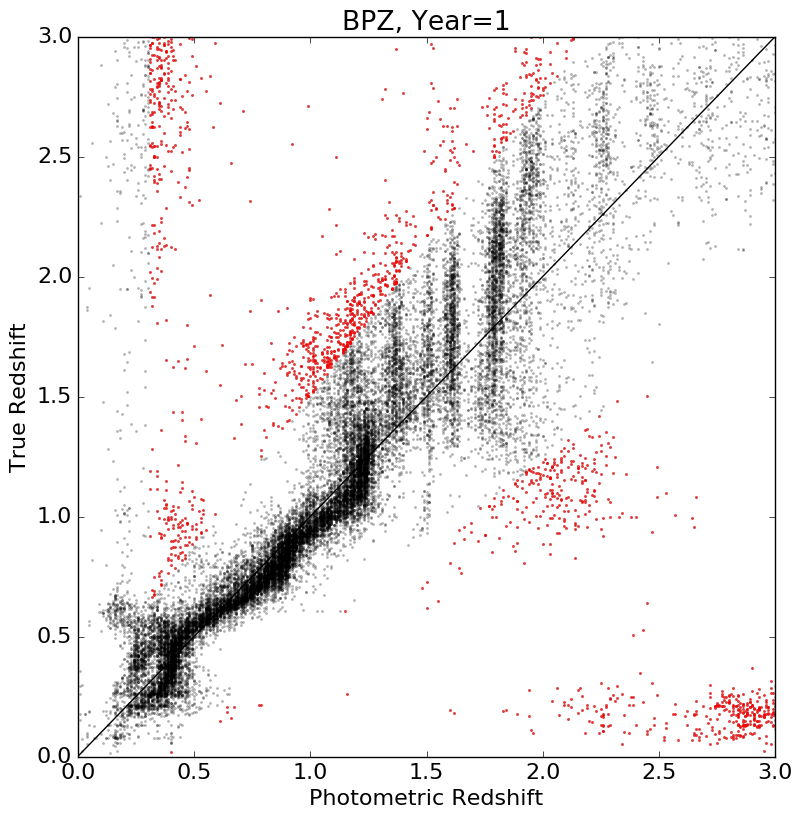
\includegraphics[width=4.0cm]{figures/BPZ_Euclid_Y1_tzpz.png}
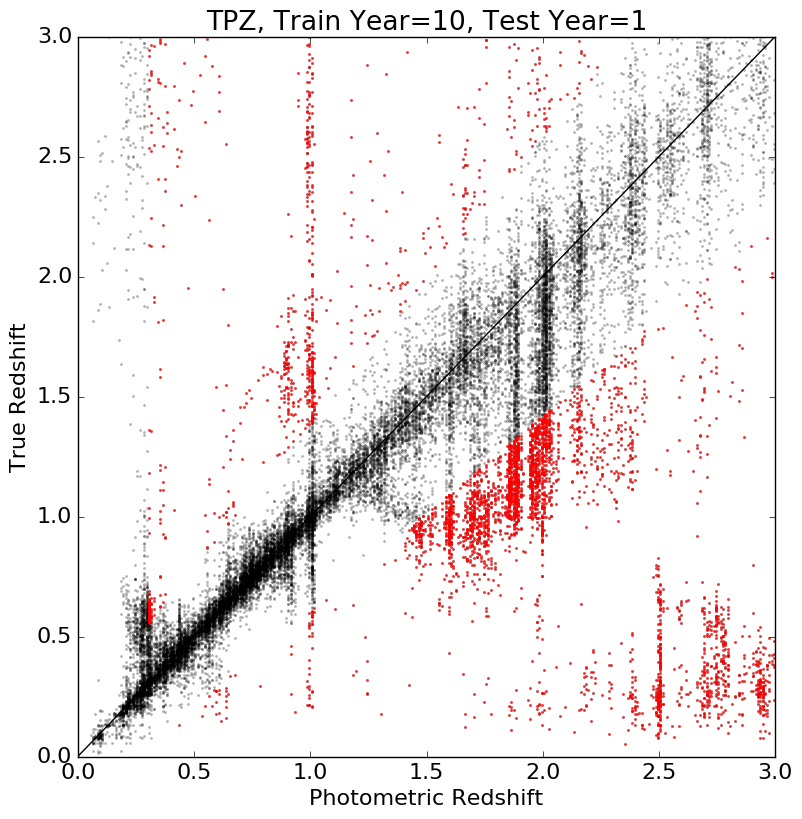
\includegraphics[width=4.0cm]{figures/TPZ_Euclid_10Y1_tzpz.png}
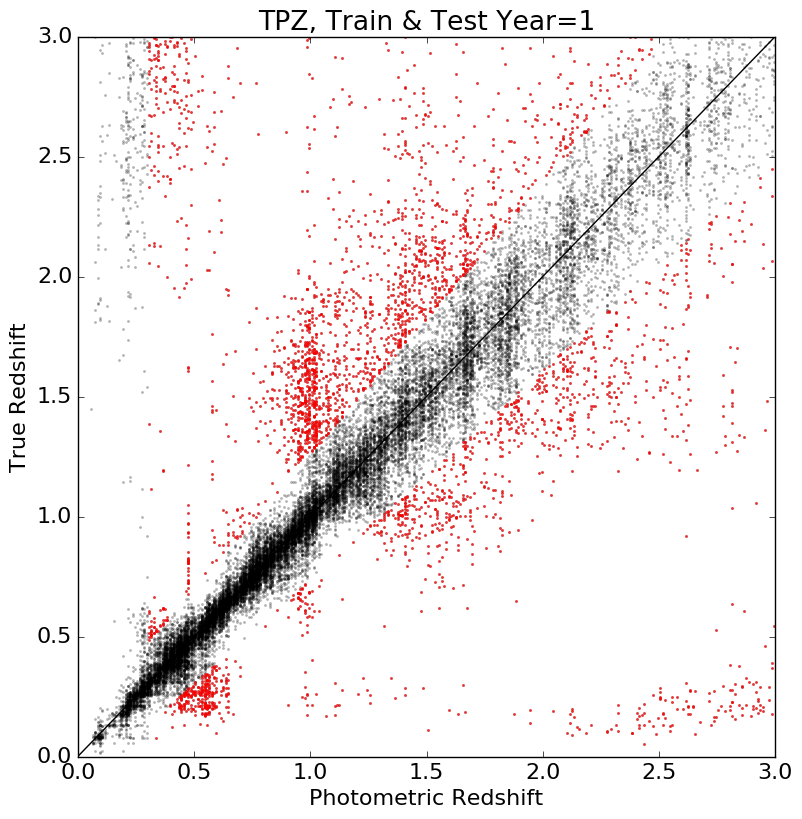
\includegraphics[width=4.0cm]{figures/TPZ_Euclid_1Y1_tzpz.png}
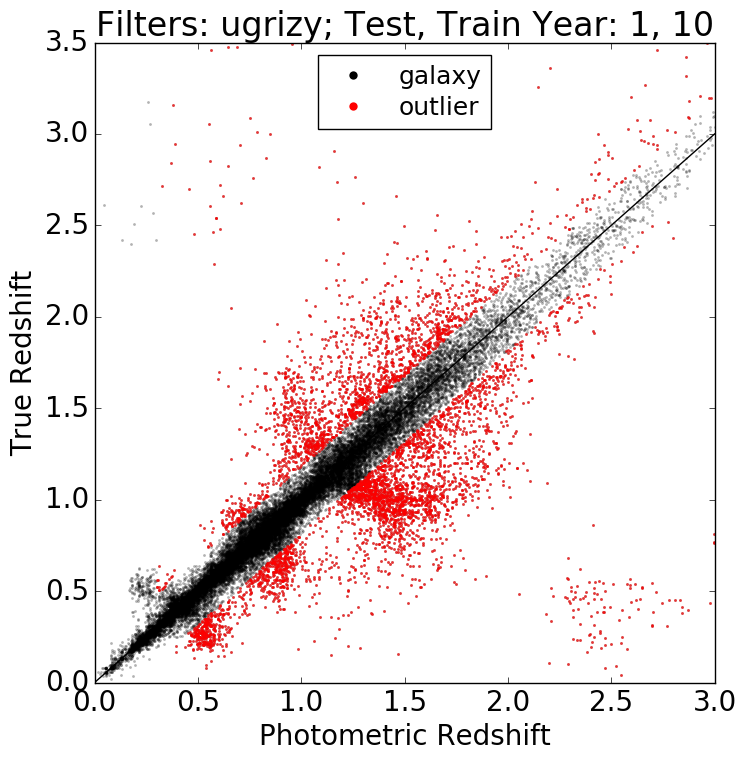
\includegraphics[width=4.0cm]{figures/CM_10Y1_tzpz.png}
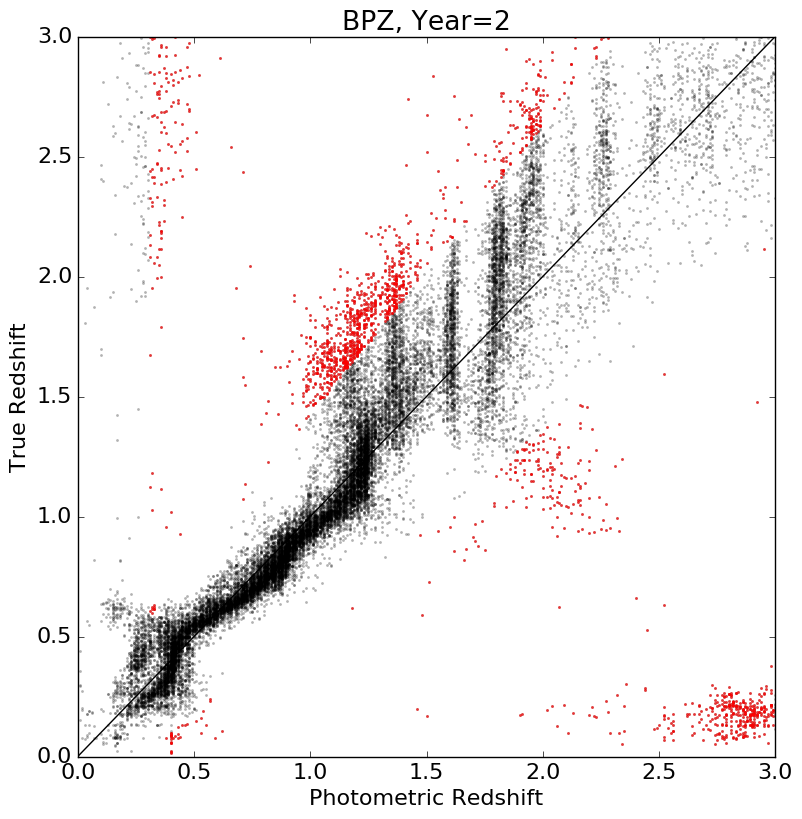
\includegraphics[width=4.0cm]{figures/BPZ_Euclid_Y2_tzpz.png}
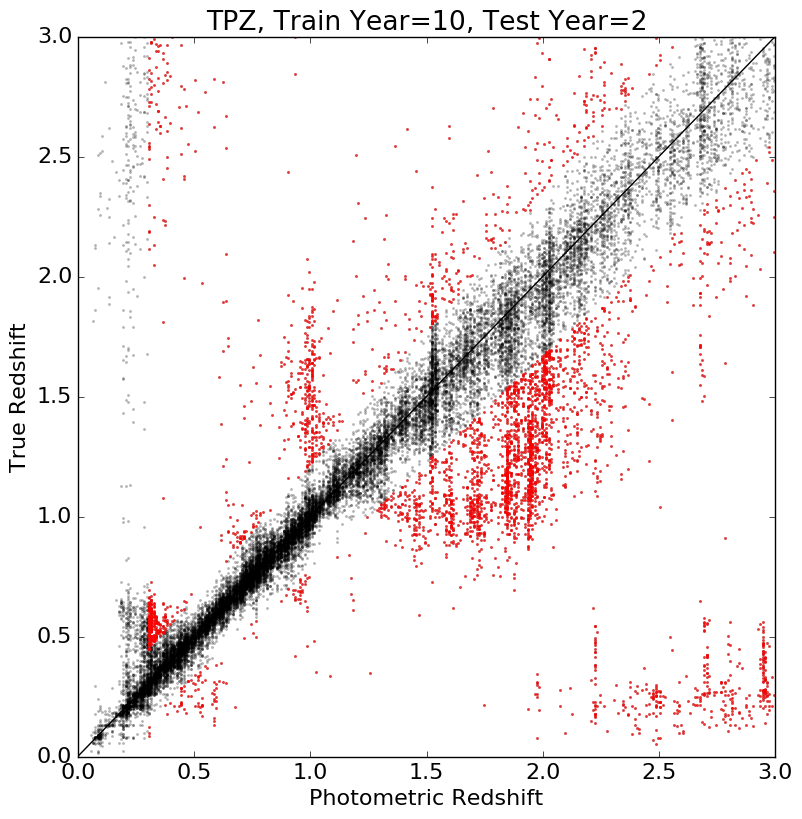
\includegraphics[width=4.0cm]{figures/TPZ_Euclid_10Y2_tzpz.png}
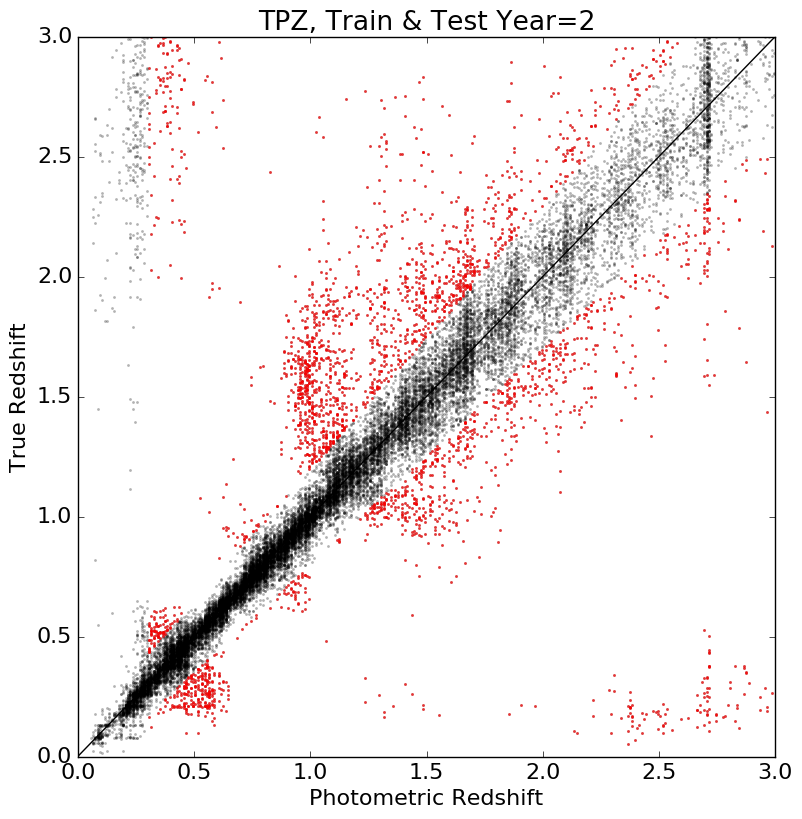
\includegraphics[width=4.0cm]{figures/TPZ_Euclid_2Y2_tzpz.png}
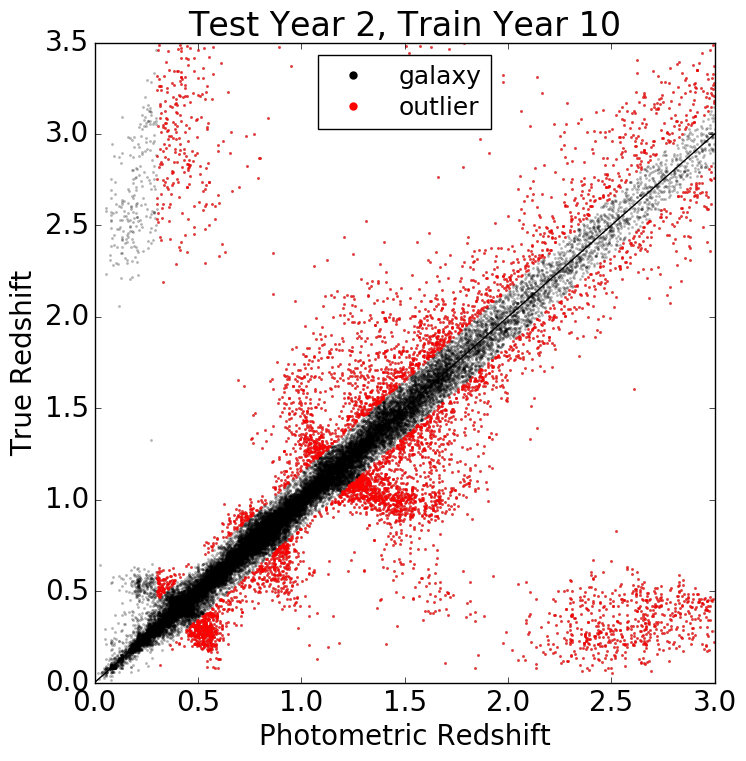
\includegraphics[width=4.0cm]{figures/CM_10Y2_tzpz.png}
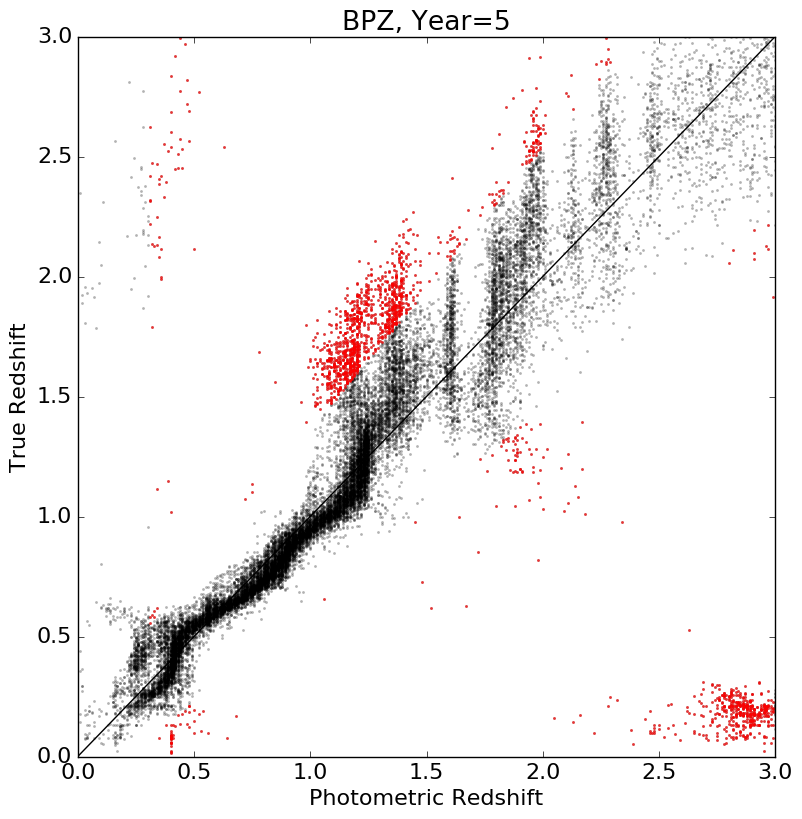
\includegraphics[width=4.0cm]{figures/BPZ_Euclid_Y5_tzpz.png}
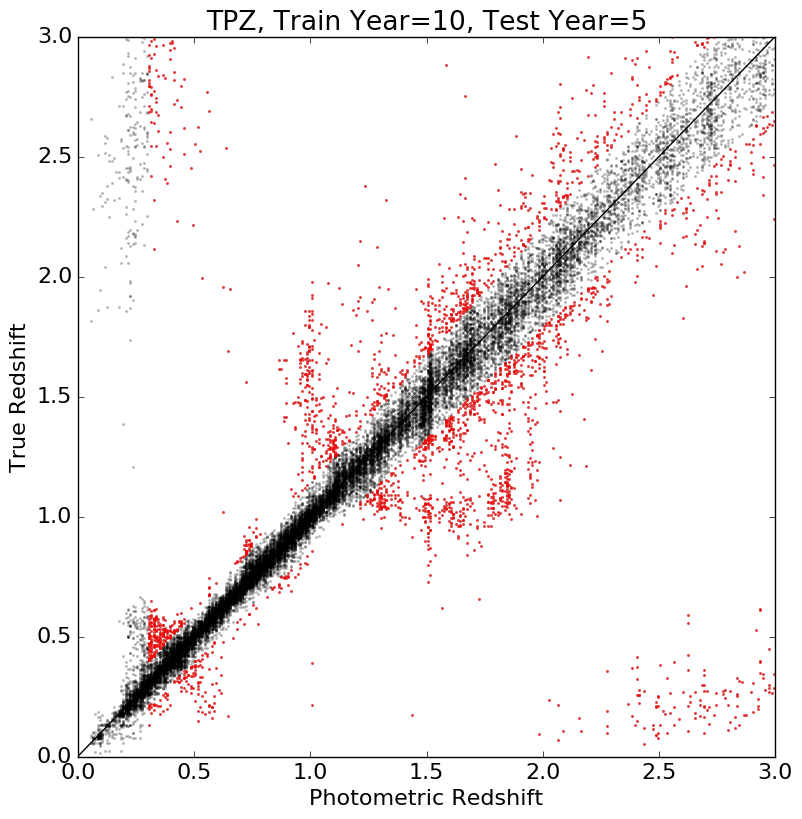
\includegraphics[width=4.0cm]{figures/TPZ_Euclid_10Y5_tzpz.png}
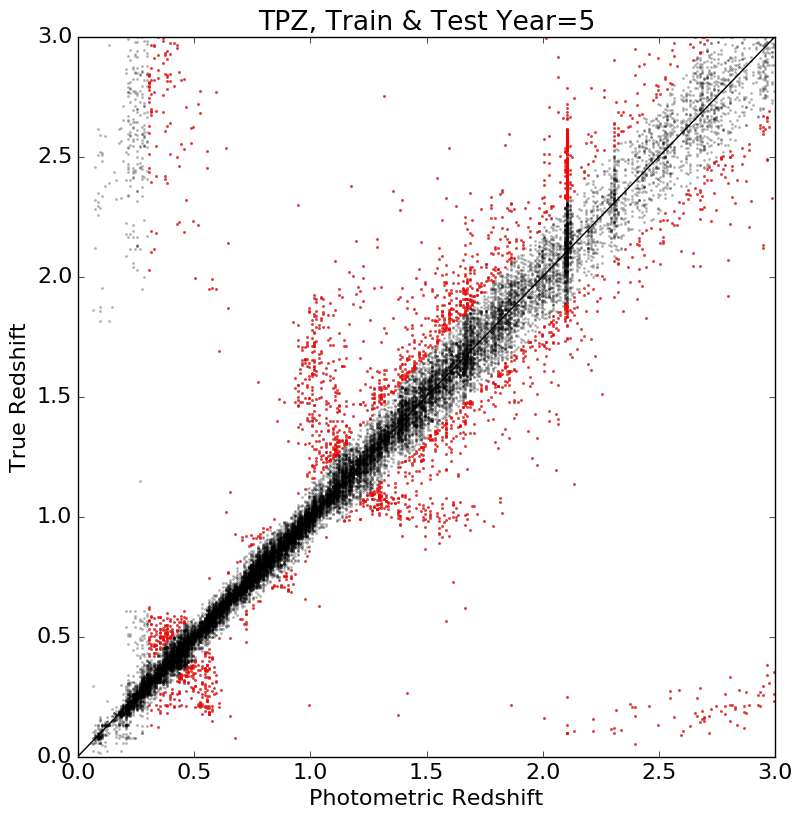
\includegraphics[width=4.0cm]{figures/TPZ_Euclid_5Y5_tzpz.png}
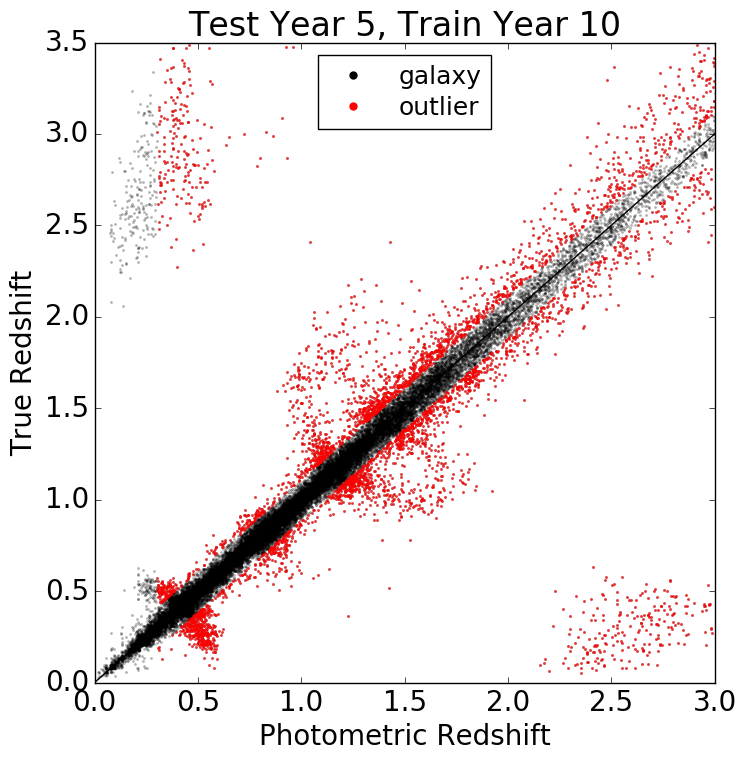
\includegraphics[width=4.0cm]{figures/CM_10Y5_tzpz.png}
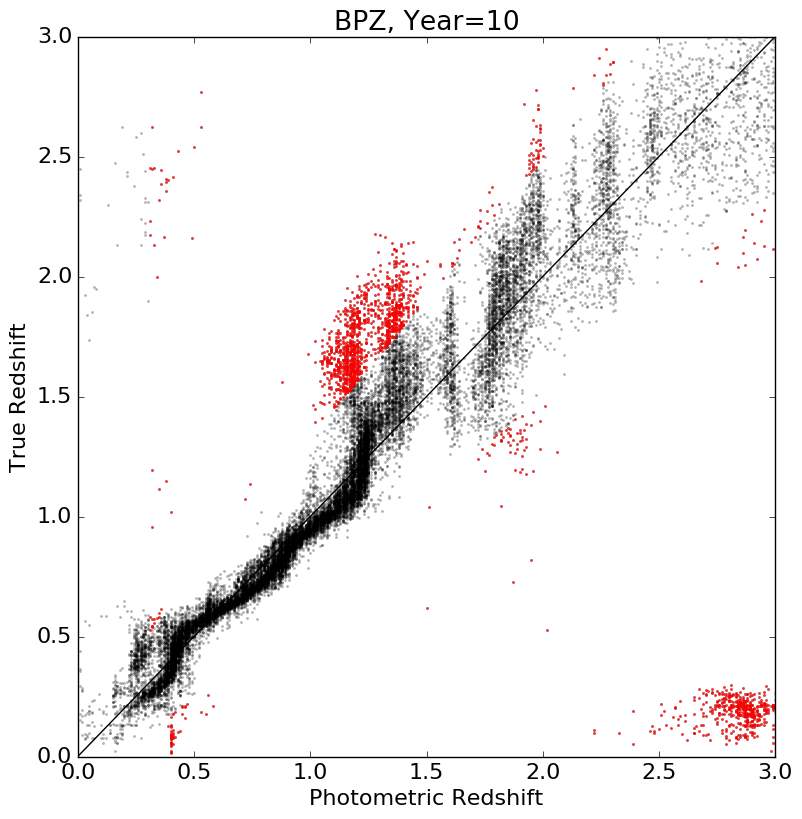
\includegraphics[width=4.0cm]{figures/BPZ_Euclid_Y10_tzpz.png}
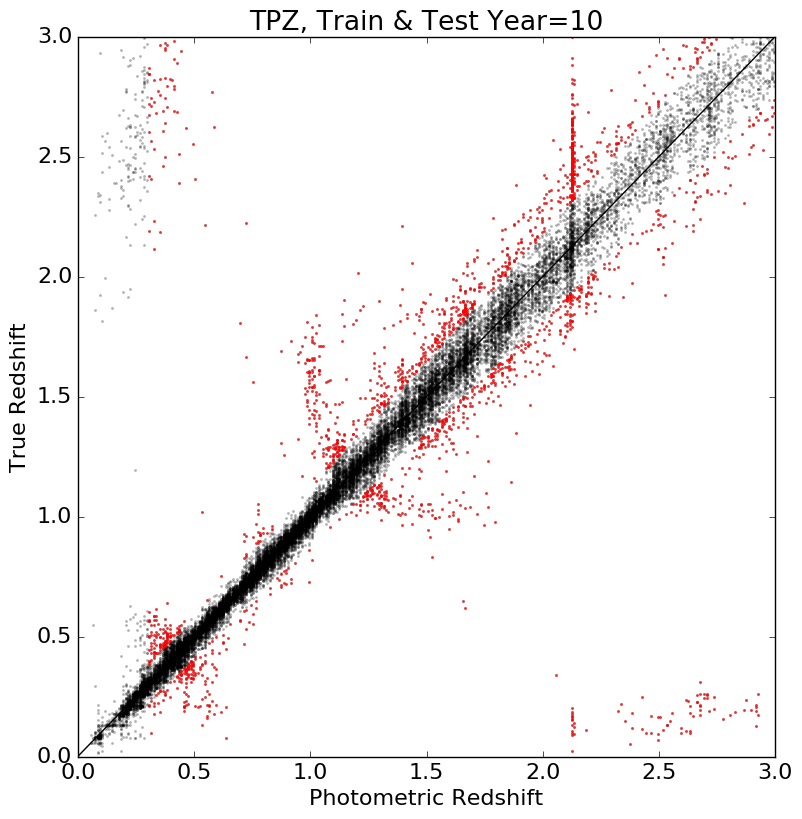
\includegraphics[width=4.0cm]{figures/TPZ_Euclid_10Y10_tzpz.png}
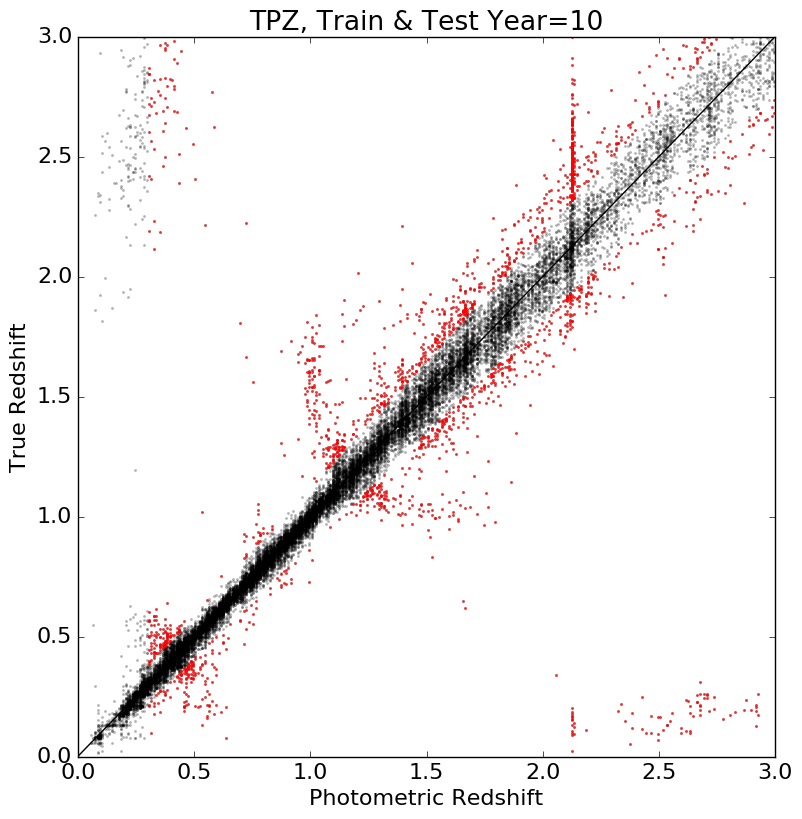
\includegraphics[width=4.0cm]{figures/TPZ_Euclid_10Y10_tzpz.png}
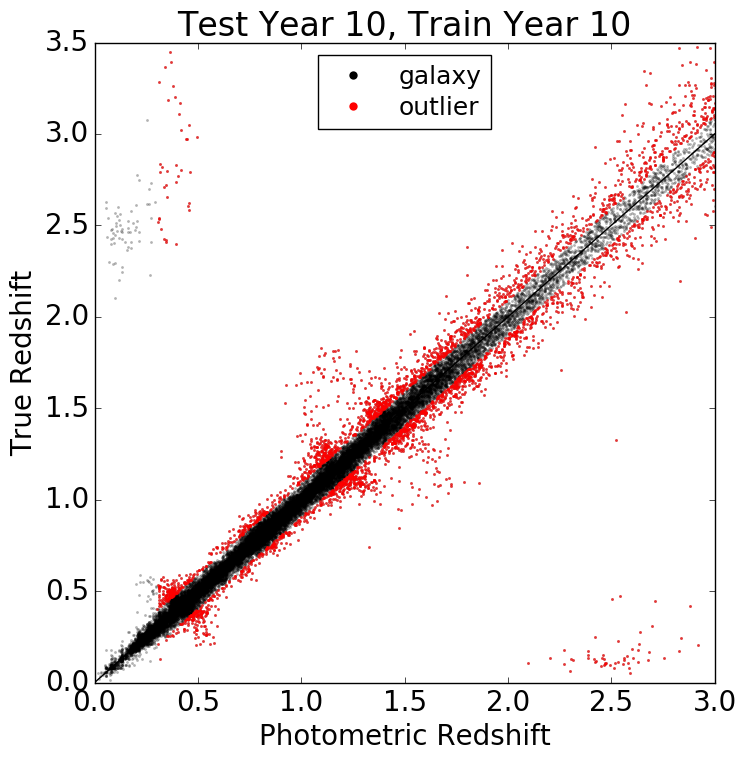
\includegraphics[width=4.0cm]{figures/CM_10Y10_tzpz.png}
\caption{Examples of $z_\mathrm{true}$--$z_\mathrm{phot}$ plots for a variety of algorithms (by column), for 1, 2, 5, or 10 years of survey time elapsed (top to bottom). Galaxies that are statistical outliers are shown in red. \textbf{Left:} results for the BPZ algorithm. \textbf{Center-left:} results for the TPZ algorithm with a 10-year training set. \textbf{Center-right:} results for the TPZ algorithm with a co-evolving training set. \textbf{Right:} results for nearest-neighbors color-matching algorithm, with 50000 test galaxies and $10^6$ training set galaxies with co-evolving photometric errors. \label{fig:tzpz}}
\end{center}
\end{figure*}

\begin{figure*}
\begin{center}
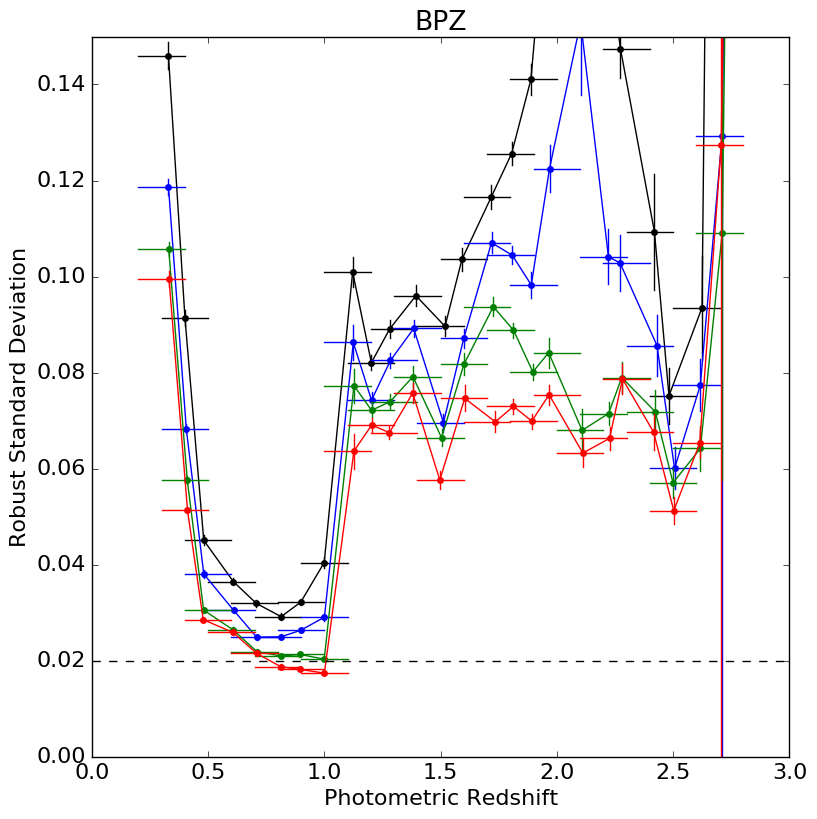
\includegraphics[width=6cm]{figures/BPZ_Euclid_IQRs.png}
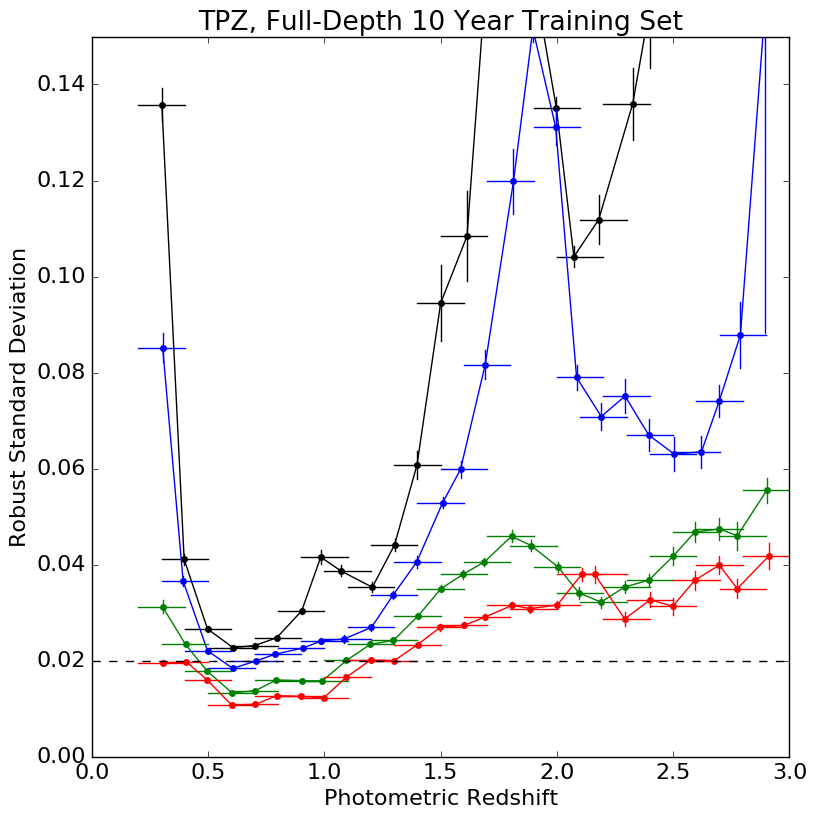
\includegraphics[width=6cm]{figures/TPZ_Euclid_TFD_IQRs.png}
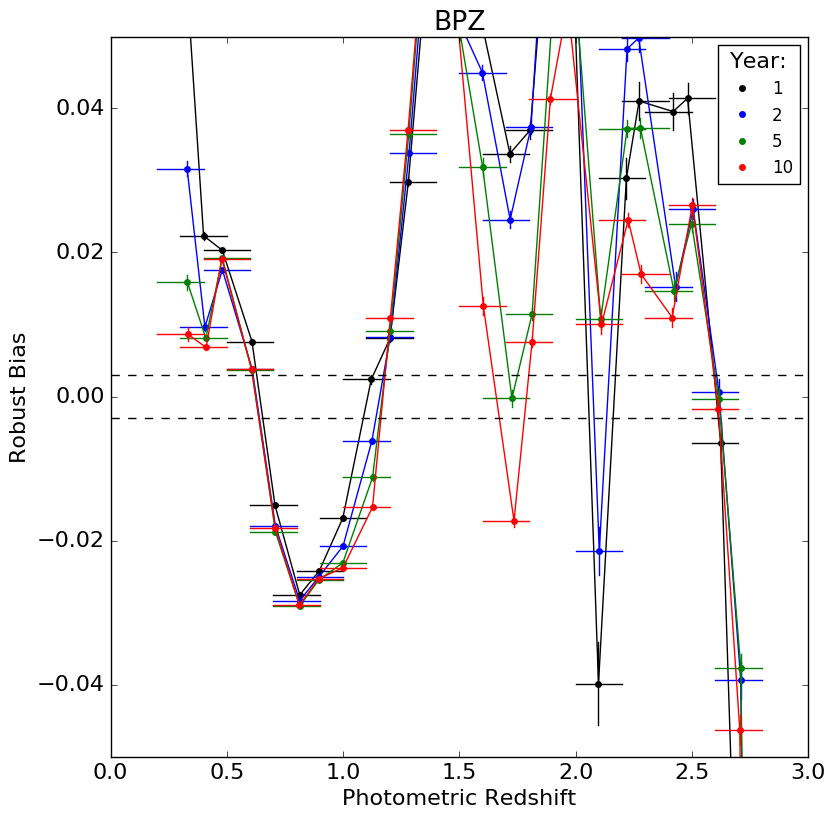
\includegraphics[width=6cm]{figures/BPZ_Euclid_bias.png}
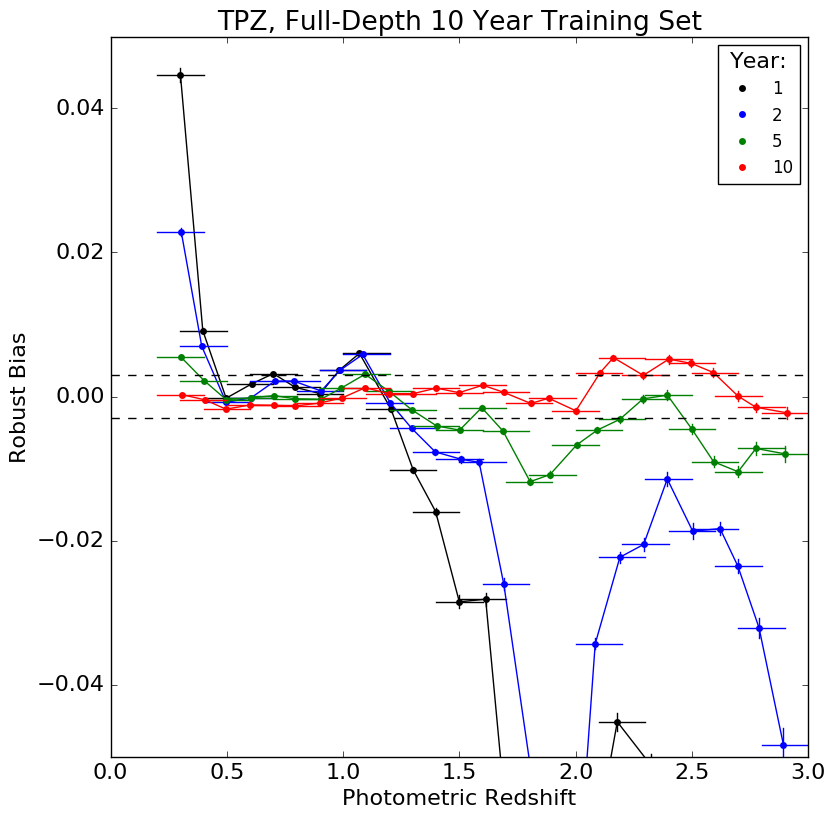
\includegraphics[width=6cm]{figures/TPZ_Euclid_TFD_bias.png}
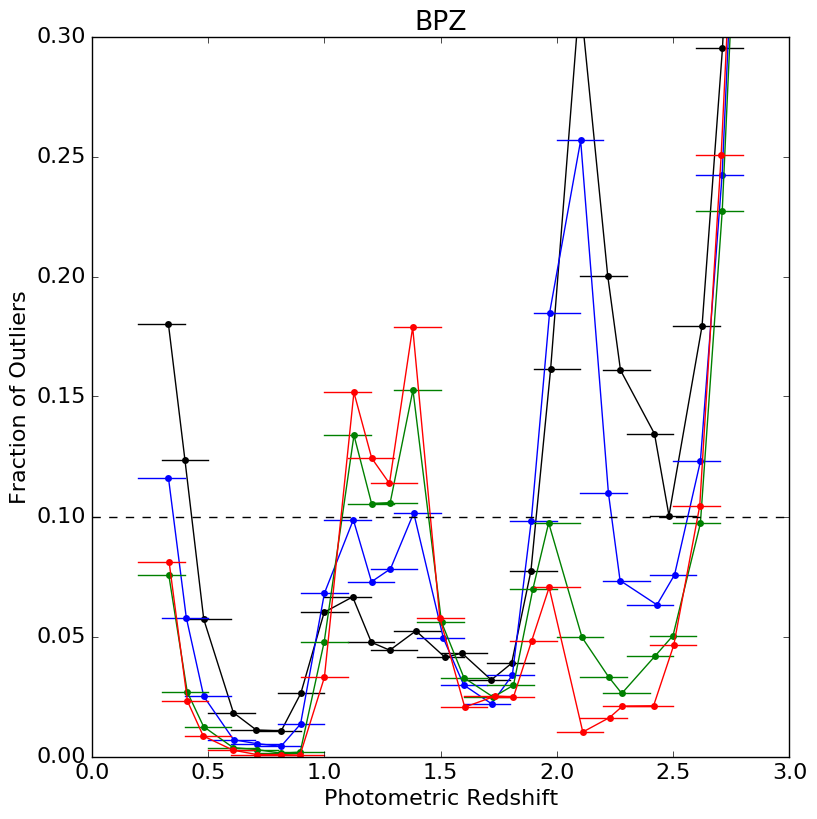
\includegraphics[width=6cm]{figures/BPZ_Euclid_fout.png}
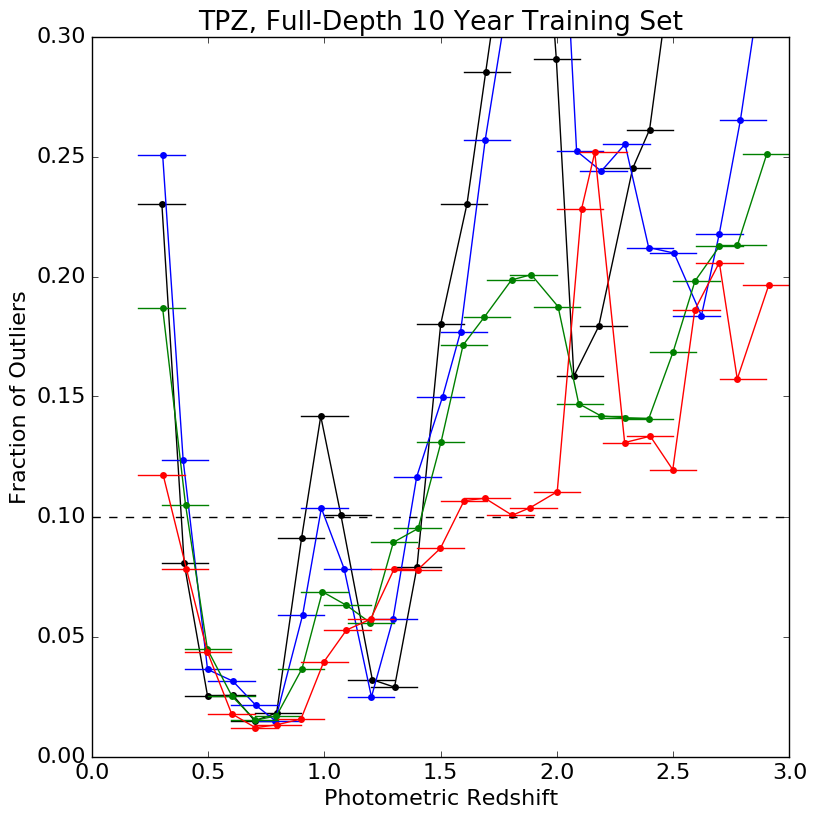
\includegraphics[width=6cm]{figures/TPZ_Euclid_TFD_fout.png}
\caption{Examples of a statistical measures of the photo-$z$ results from BPZ (left) and TPZ with an evolving training set (right) for simulated catalogs at 1 to 10 years (line colors as in plot legends). From top to bottom we show the robust standard deviation from the IQR, the robust bias, and the fraction of outliers as a function of photo-$z$, with matched $x$- and $y$-axes to facilitate comparison between BPZ and TPZ. \label{fig:stats}}
\end{center}
\end{figure*}

\begin{figure*}
\begin{center}
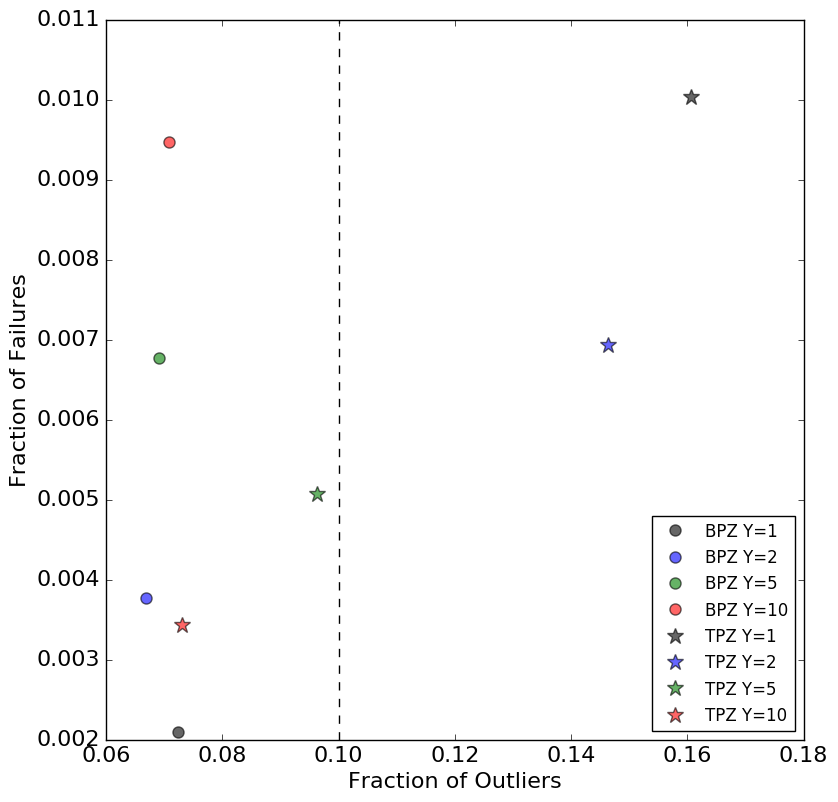
\includegraphics[width=8cm]{figures/stat_stat_fout_ffail.png}
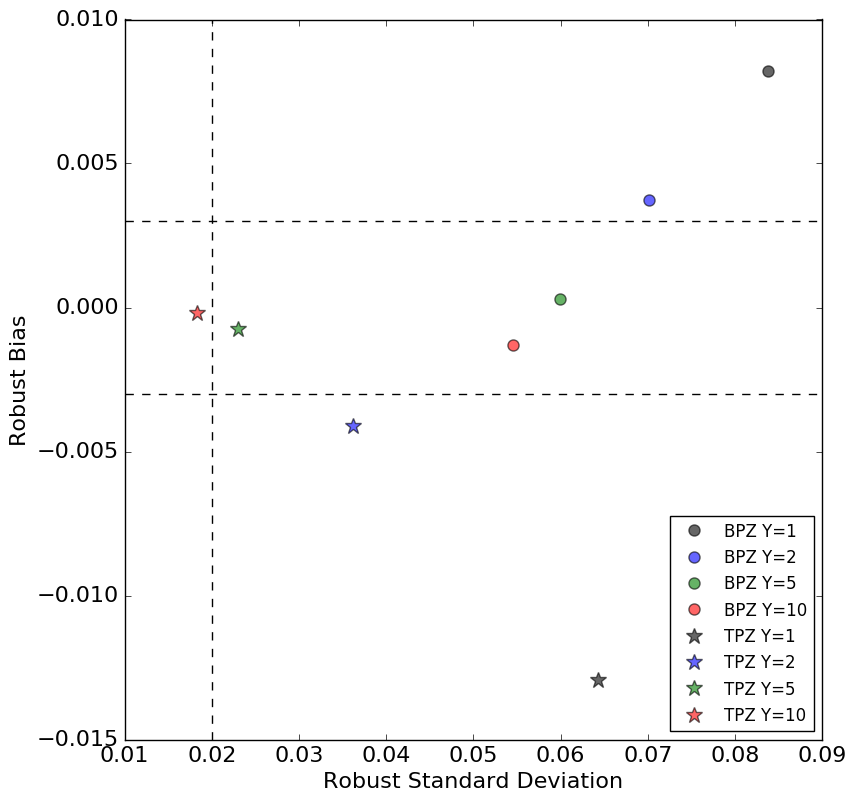
\includegraphics[width=8cm]{figures/stat_stat_std_bias.png}
\caption{Examples of how to compare statistical measures over $0.3 \leq z_\mathrm{phot} \leq 3.0$ from different photo-$z$ estimators by plotting one against the other: fraction of failures and outliers (left), and the robust bias and standard deviation (right). In this case we're comparing the statistical measures for TPZ and BPZ from photometry simulated for the LSST at years 1, 2, 5, and 10 (legend).  \label{fig:stat_stat}}
\end{center}
\end{figure*}

\begin{figure*}
\begin{center}
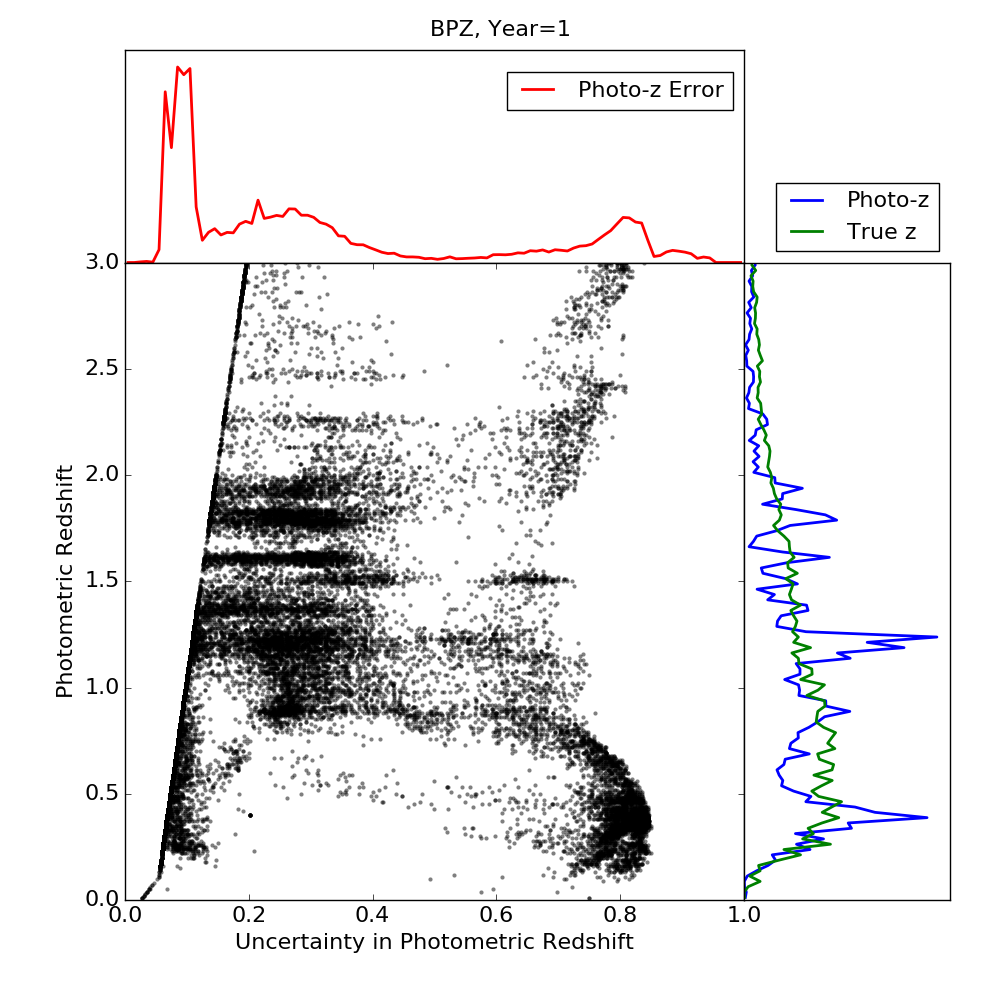
\includegraphics[width=6cm,trim={1cm 1cm 1cm 0cm}, clip]{figures/zp_zpe_bpz_euclid_1_2.png}
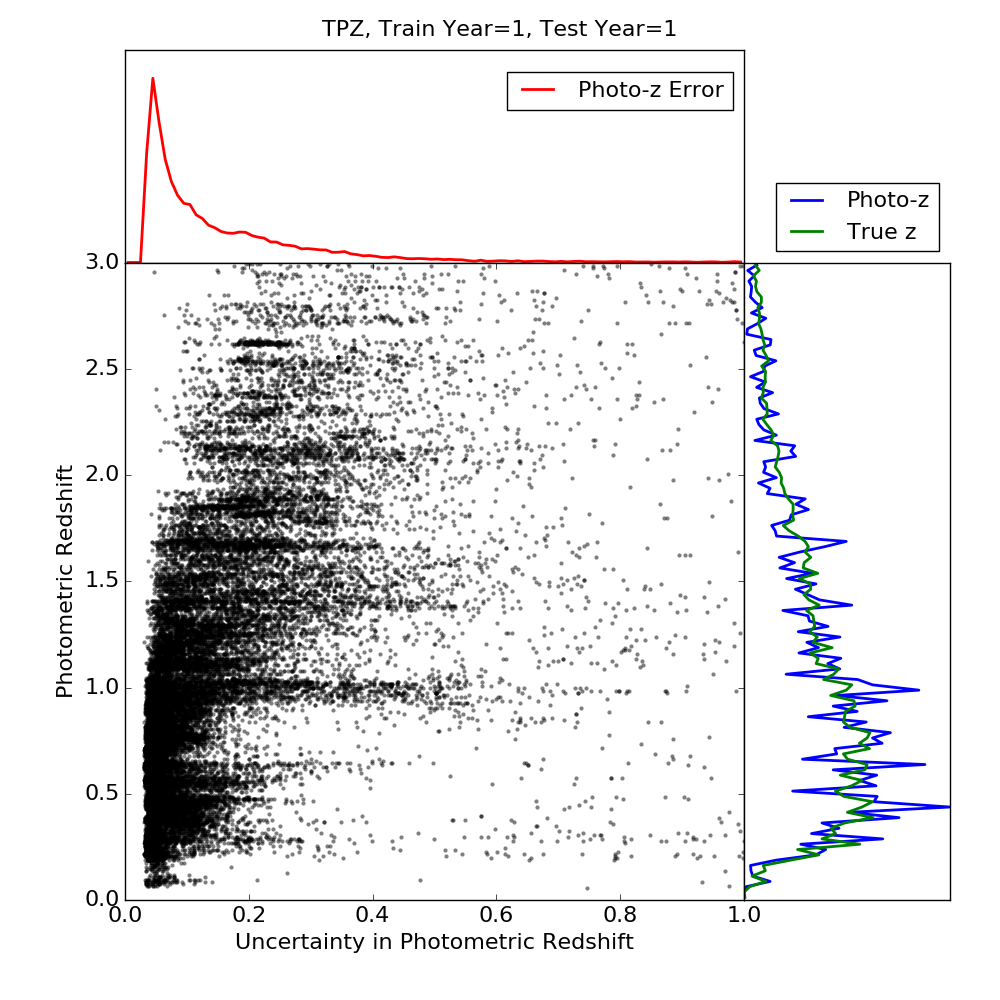
\includegraphics[width=6cm,trim={1cm 1cm 1cm 0cm}, clip]{figures/zp_zpe_tpz_euclid_1_1_2.png}
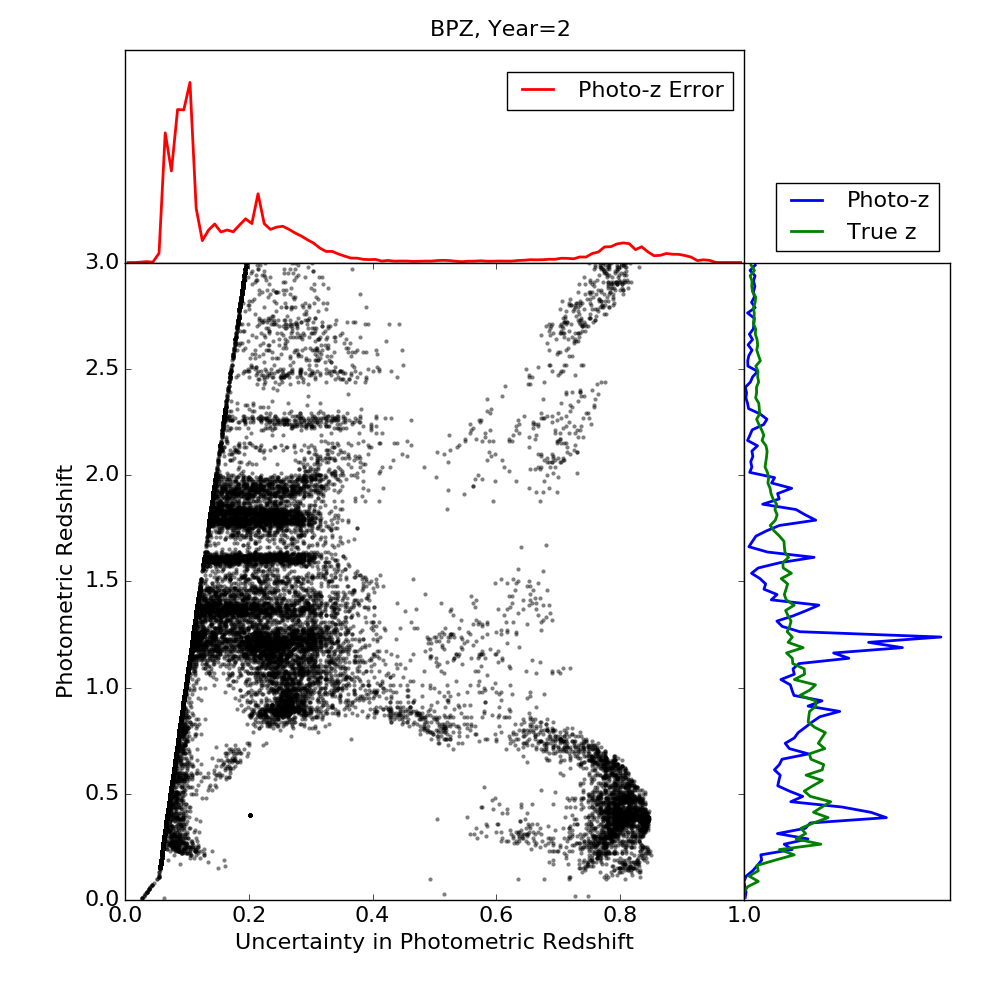
\includegraphics[width=6cm,trim={1cm 1cm 1cm 0cm}, clip]{figures/zp_zpe_bpz_euclid_2_2.png}
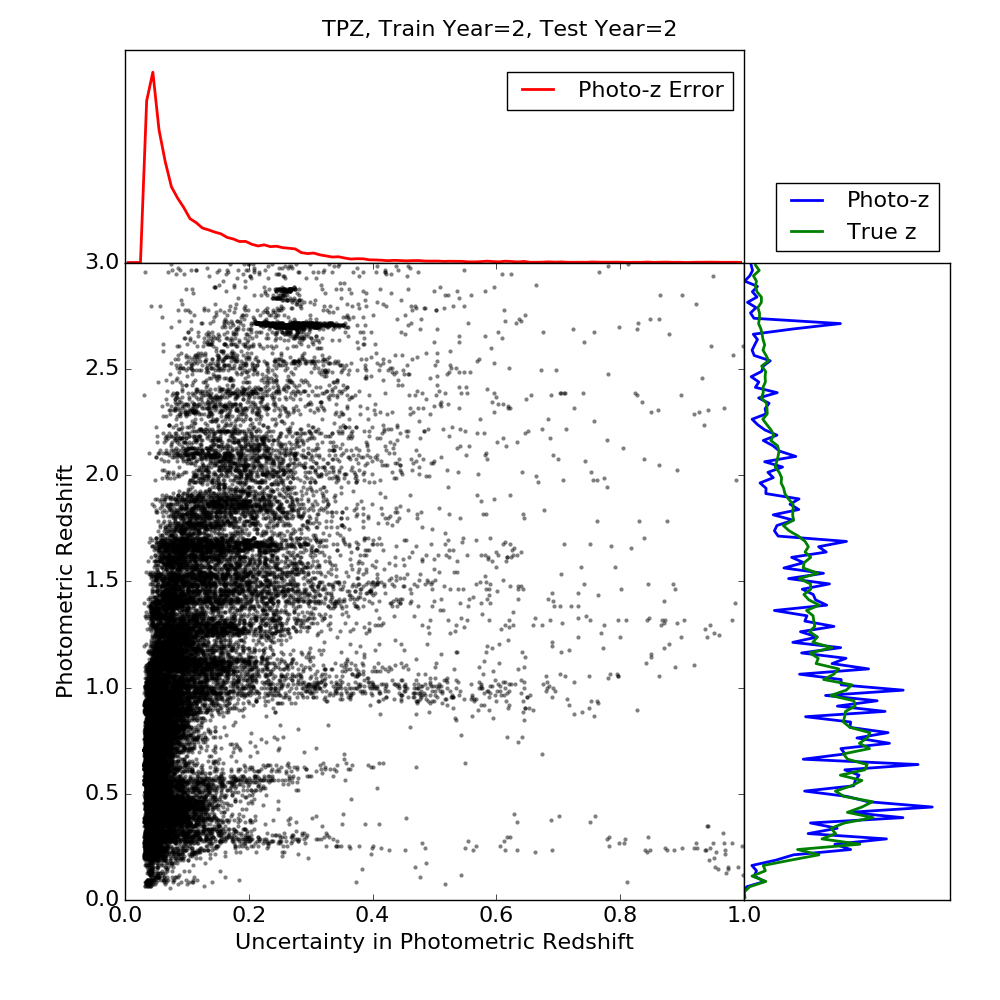
\includegraphics[width=6cm,trim={1cm 1cm 1cm 0cm}, clip]{figures/zp_zpe_tpz_euclid_2_2_2.png}
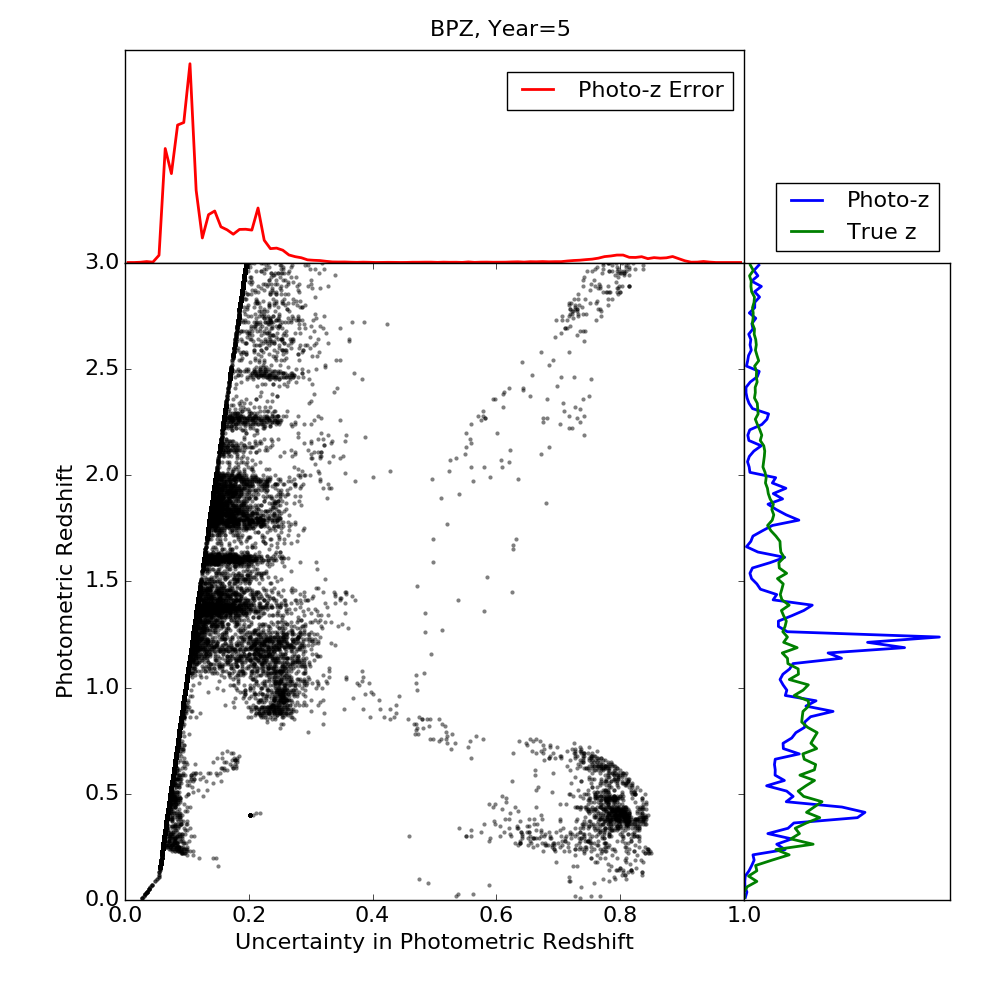
\includegraphics[width=6cm,trim={1cm 1cm 1cm 0cm}, clip]{figures/zp_zpe_bpz_euclid_5_2.png}
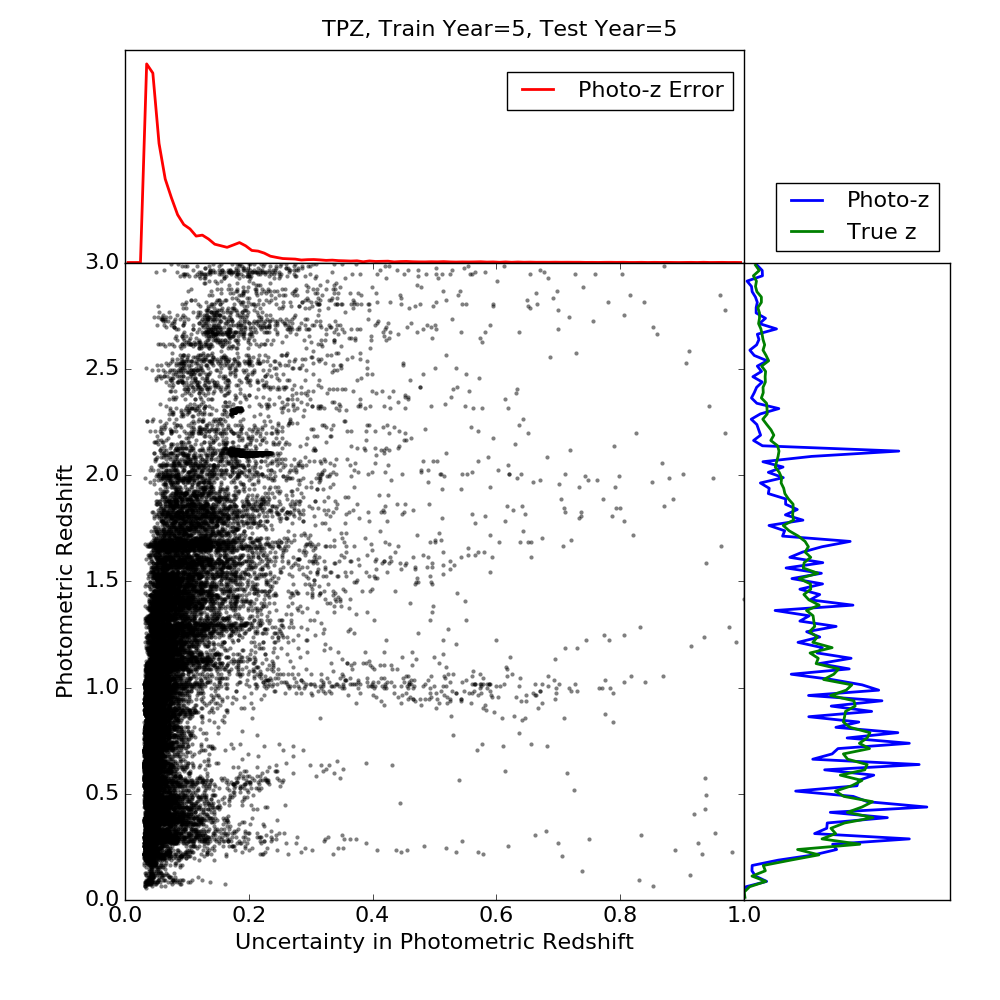
\includegraphics[width=6cm,trim={1cm 1cm 1cm 0cm}, clip]{figures/zp_zpe_tpz_euclid_5_5_2.png}
\caption{Examples of plot to compare the photo-$z$ uncertainty ($\delta z_\mathrm{phot}$) between algorithms with $z_\mathrm{phot}$--$\delta z_\mathrm{phot}$ plots from the BPZ (left) and TPZ (right) estimators for simulated catalogs with photometric uncertainties at 1, 2, and 5 years of LSST (top to bottom). Red lines show the distribution of photo-$z$ errors; blue and green lines compare the distributions of true and photometric redshifts. \label{fig:pzpze}}
\end{center}
\end{figure*}

\begin{figure*}
\begin{center}
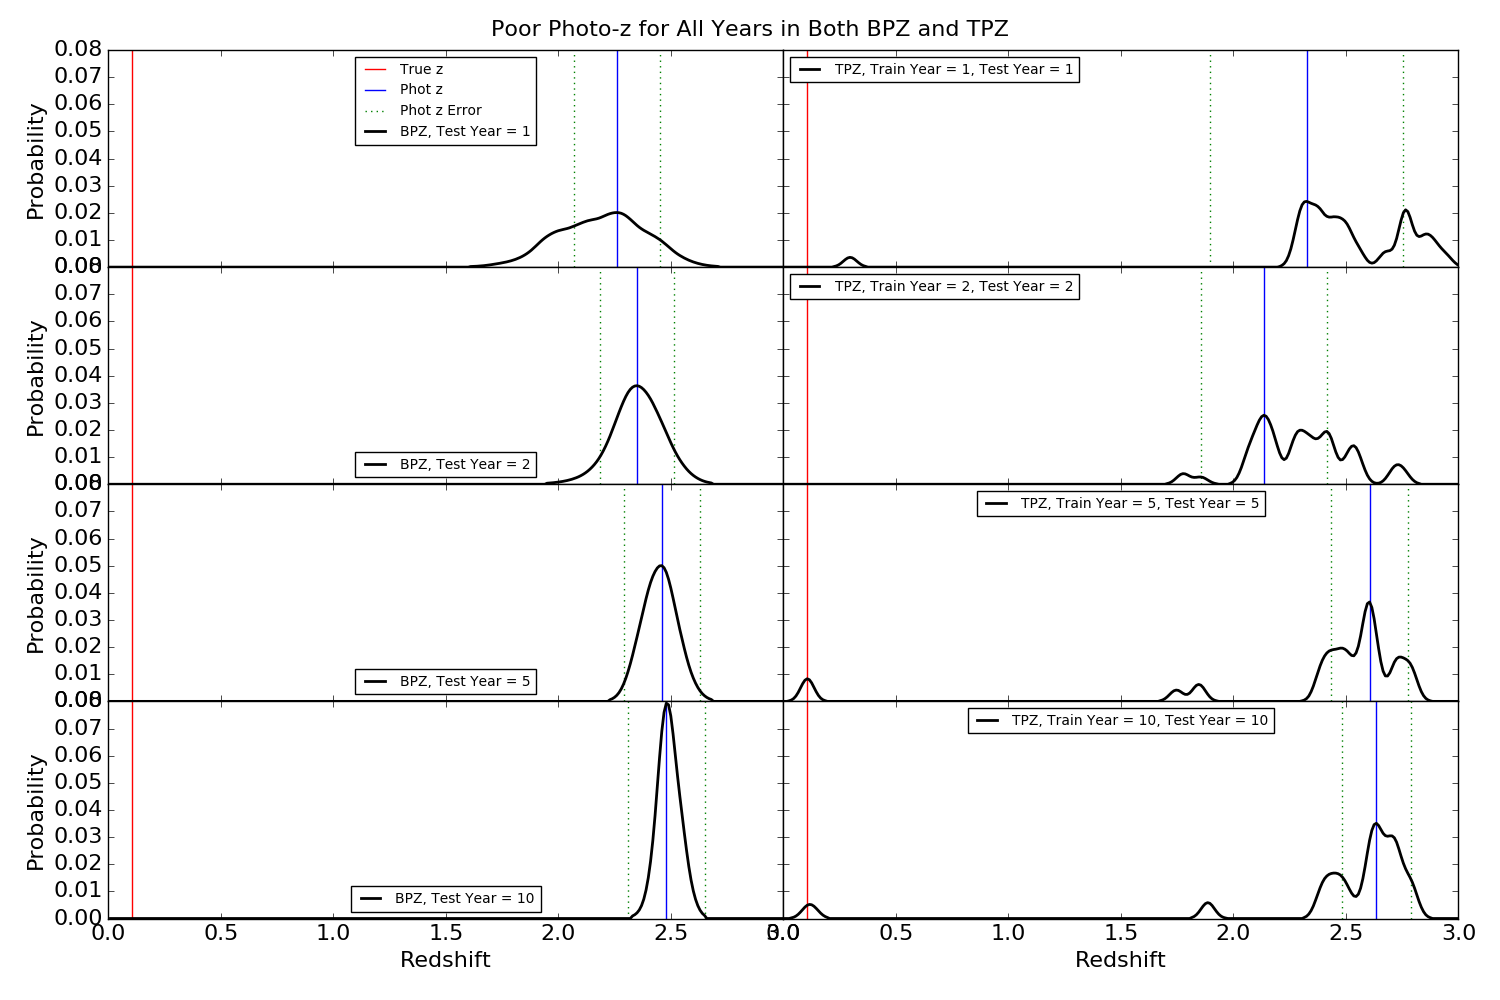
\includegraphics[width=13cm]{figures/zpdf_g4.png}
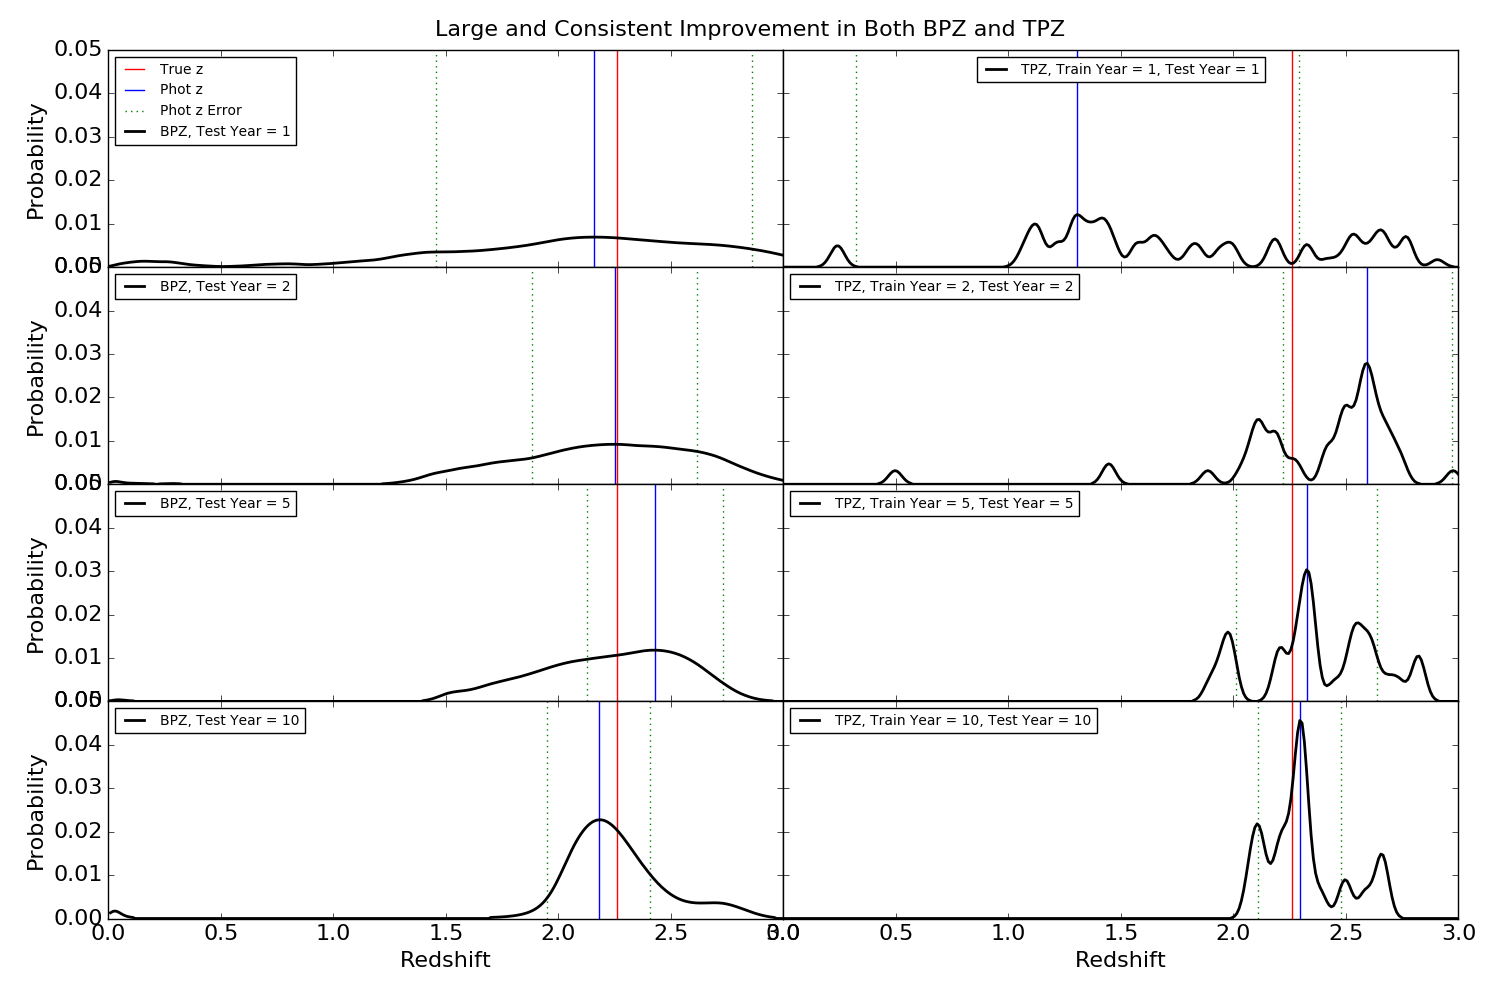
\includegraphics[width=13cm]{figures/zpdf_g7.png}
\caption{Examples of the posterior probability density functions for two test galaxies in all of our simulations: BPZ (left) and TPZ (right) for photometric uncertainties like 1, 2, 5, and 10 years of LSST (rows from top to bottom). In the top panel we choose a galaxy that return inaccurate and imprecise photo-$z$ from all 8 trials, and in the bottom panel we choose a galaxy that experienced a large and consistent improvement in photo-$z$ accuracy and precision from 1 to 10 years with both estimators.  \label{fig:zpdf}}
\end{center}
\end{figure*}

\begin{figure*}
\begin{center}
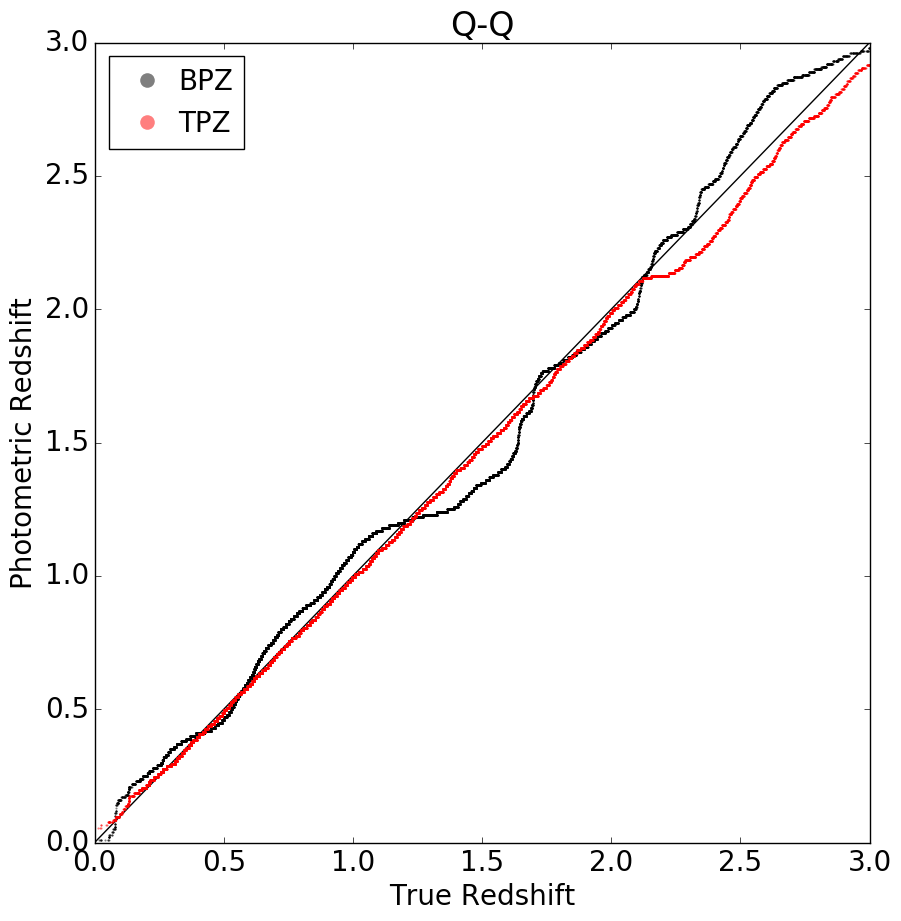
\includegraphics[width=10cm]{figures/qq_BPZ_TPZ.png}
\caption{Example of a Q-Q plot, using $z_\mathrm{true}$ and $z_\mathrm{phot}$, from the BPZ and TPZ estimators.}\label{fig:qq}
\end{center}
\end{figure*}

\clearpage

\bibliography{lsst,refs_ads,local}

\end{document}
